%package obligatoire : type de document
\documentclass[a4paper,12pt,twoside]{book}
\usepackage{lipsum}

% encodage
\usepackage{fontspec}

% le package hyperref avec des options
\usepackage[pdfusetitle, pdfsubject ={Mémoire TNAH - Numérisation d'un référentiel papier pour indéxation automatique}, pdfkeywords={TNAH, IRHT, Himanis, Trésor des Chartes, Archives Nationales, ROC, Numérisation d'instruments de recherche, Alignement de référentiels, REM, REN, Machine learning, Intelligence artificielle, Reconnaissance d'écritures manuscrites, identity linking}, hidelinks]{hyperref}

%il faut mettre au moins une langue
\usepackage[english,french]{babel}

% configurer le document selon les normes de l'école
\usepackage[margin=2.5cm]{geometry} %marges
\usepackage{setspace} % espacement qui permet ensuite de définir un interligne
\onehalfspacing % interligne de 1.5
\setlength\parindent{1cm} % indentation des paragraphes à 1 cm
\parskip=5pt %Crée un espace entre les paragraphes pour aérer le texte

\usepackage{lettrine} % lettrines

%Pour importer des images
\usepackage{subcaption}
\usepackage{graphicx}
\usepackage{float}
\usepackage{chngcntr}
\counterwithout{figure}{chapter} % Pour que les images ne soient pas comptées en fonction des chapitres
\DeclareCaptionFormat{custom}
{%
	\textbf{#1#2}\textit{\small #3}
}
\captionsetup{format=custom} % Améliore le format de légende des images

\pagestyle{plain} % Pour une numérotation des pages sobre

\usepackage[backend=bibtex, sorting=nyt, style=enc]{biblatex}
\FrenchFootnotes
\AddThinSpaceBeforeFootnotes
\addbibresource{Mémoire-TNAH-2022-Reignier.bib}

\author{Virgile Reignier - M2 TNAH}
\title{Vers l’indexation automatique du Trésor des chartes. Constitution, alignement et utilisation de référentiels d’entités nommées au sein du projet Himanis.}

\makeatletter
\newcommand{\parttext}[1]{\def\@parttext{#1}}
\def\@endpart{\vskip 0pt plus 0.5fil
	\begin{formatparttext}
		\vspace*{\fill}
		\@parttext % on imprime le texte spécifique à une partie
		\gdef\@parttext{}% on vide le texte spécifique à une partie
		\vspace*{\fill}
	\end{formatparttext}
	\vskip 0pt plus 0.5fil
	\newpage
	\if@twoside
	\if@openright
	\null
	\thispagestyle{empty}%
	\newpage
	\fi
	\fi
	\if@tempswa
	\twocolumn
	\fi}
\makeatother

\newenvironment{formatparttext}{}{}

% DOCUMENT
\begin{document}
	\begin{titlepage}
		\begin{center}
			
			\bigskip
			
			\begin{large}				
				ÉCOLE NATIONALE DES CHARTES\\
				UNIVERSITÉ PARIS, SCIENCES \& LETTRES
			\end{large}
			\begin{center}\rule{2cm}{0.02cm}\end{center}
			
			\bigskip
			\bigskip
			\bigskip
			\begin{Large}
				\textbf{Virgile Reignier}\\
			\end{Large}
			%selon le cas
			\begin{normalsize} \textit{licencié.e ès histoire}\\
				\textit{diplômé.e de master mondes médiévaux}
			\end{normalsize}
			
			\bigskip
			\bigskip
			\bigskip
			
			\begin{Huge}
				\textbf{Vers l’indexation automatique du Trésor des chartes}\\
			\end{Huge}
			\bigskip
			\bigskip
			\begin{LARGE}
				\textbf{Constitution, alignement et utilisation de référentiels d’entités nommées au sein du projet Himanis}\\
			\end{LARGE}
			
			\bigskip
			\bigskip
			\bigskip
			\begin{large}
			\end{large}
			\vfill
			
			\begin{large}
				Mémoire 
				pour le diplôme de master \\
				\og{} Technologies numériques appliquées à l'histoire \fg{} \\
				\bigskip
				2022
			\end{large}
			
		\end{center}
	\end{titlepage}
	
	\thispagestyle{empty}	
	\cleardoublepage
	
	\frontmatter
	\chapter{Résumé}
	\medskip
	Blablabla résumé du mémoire.\\
	
	\textbf{Mots-clés~:} TNAH, IRHT, Himanis, Trésor des Chartes, Archives Nationales, ROC, Numérisation d'instruments de recherche, Alignement de référentiels, REM, REN, Machine learning, Intelligence artificielle, Reconnaissance d'écritures manuscrites, identity linking.
	
	\textbf{Informations bibliographiques~:} Reignier Virgile, \textit{Vers l’indexation automatique du Trésor des chartes. Constitution, alignement et utilisation de référentiels d’entités nommées au sein du projet Himanis.}, mémoire de master \og{}Technologies numériques appliquées à l'histoire\fg{}, dir. Dominique Stutzmann et Thibault Clérice, École nationale des chartes, 2022.
	
	\chapter{Remerciements}
	
	\lettrine{B}lablabla remerciements\dots
	
		Faire une liste des abréviations avec : REN, TAL, REM, IRHT, BVMM, EAD, TEI, XML, XSL, CNRS
	
	\printbibliography
	
	\chapter{Introduction}
	
	\begin{quotation}
		
	A ce sujet papa avait une plaisanterie. (...) Il disait, quand il présentait maman, « je l’ai connue et épousée à Paris » et (...) il attendait avant de dire « Texas » que tout le monde ait cru, que tout le monde ait pensé qu’il parlait de Paris, France. Ça faisait tordre de rire toutes les fois.
	
	\end{quotation}
	\bigbreak
	
	
	\lettrine{S}{i} le mot "Paris" évoque en premier lieu la capitale française, il désigne également d'autres villes à travers le monde. C'est en exploitant l'homonymie entre cette première et une ville du Texas que la citation ci-dessus, extraite du film "Paris, Texas" (1984) de Wim Wenders, construit la plaisanterie. L'information "Paris" ne suffit en effet pas à identifier le lieu où lesdits parents se sont rencontrés. Utilisé seul, le mot est naturellement associé à la France. C'est seulement en précisant l'État dans lequel la ville se situe que l'on peut identifier le lieu exact où les protagonistes se sont rencontrés et mariés. Ce jeu d'ambiguïté manifeste ainsi d'une difficulté rencontrée dans le langage naturel : l'identification des références utilisées. La connaissance lexicale ne suffit en effet pas à elle seule pour comprendre un discours, il faut également que les références soient comprises et associées à une réalité clairement identifiée.
	
	Cet enjeu est également présent au sein du TAL (Traitement Automatique des Langues) à travers la notion d'Entité Nommée qui désigne une expression linguistique qui se réfère à une entité unique de façon autonome\footnote{Sur la définition des entités nommées, \textit{cf}. \cite[p. 167--170]{ehrmann_les_2008}.}. L'analyse du contenu textuel a ainsi largement progressé ces dernières années autour de cette notion par le développement de deux techniques : la REN (Reconnaissance d'Entités Nommées) qui consiste à repérer ces objets textuels et à leur attribuer une catégorie et le liage d'entités qui permet d'associer ces objets textuels à un élément décrit par une ressource référentielle. Si un grand nombre de ces travaux concernent des corpus contemporains, quelques chercheurs s'intéressent également à leur application pour la lecture des archives anciennes et rencontrent ainsi les recherches menées par les spécialistes de ces corpus.
	
	\subsection*{Contexte scientifique de travail}
	
	L'Institut de Recherche et d'Histoire des Textes (IRHT) est un laboratoire de recherche fondé en 1937 par Félix Grat et rattaché au CNRS dans le but de faciliter l'accès des chercheurs aux manuscrits et imprimés anciens\footnote{Sur la fondation de l'IRHT, \textit{cf}. \cite{holtz_les_2000}.}. Les recherches qui y sont menées portent également sur la transmission des textes et l'étude des écritures et connaissent à ce titre des développements récents à propos de la lecture automatique des documents anciens. Initiés par sa collaboration au sein du projet GRAPHEM, les travaux en "paléographie artificielle" développés par la section de paléographie latine sont menés conjointement avec des chercheurs en informatique spécialisés dans l'analyse de l'image. Les projets développés prennent deux directions principales : la caractérisation des écritures médiévales (Oriflamms, ECMEN, CrEMe) d'une part et la lecture automatique des archives (Himanis, HOME, HORAE) d'autre part. Pilotés par Dominique Stutzmann, ces recherches ont permis le développement d'outils informatiques et de modèles d'intelligence artificielle qui ont largement renouvelé l'accès aux textes anciens.
	
	Parmi les corpus étudiés par ces travaux, le Trésor des Chartes occupe une place centrale puisqu'il constitue le matériel source du projet Himanis et participe à celui du projet HOME. Conservé au sein de la série JJ des Archives Nationales, ce fonds se compose d'une immense collection de titres rassemblée par les rois de France. Il se présente sous la forme de registres contenant des actes organisés de manière plus ou moins systématique et linéaire\footnote{Sur la constitution du Trésor des Chartes, \textit{cf}. \cite{potin_mise_2007}}. Le projet Himanis (HIstorical MANuscript Indexing for user-controlled Search) a ainsi permis de numériser les registres et de convertir les inventaires et éditions disponibles afin de les structurer en un format homogène et unique\footnote{Les registres numérisés ont été intégrés à la Bibliothèque Virtuelle des Manuscrits Médiévaux \cite{noauthor_bvmm_nodate}. Tous les fichiers issus de ces travaux sont disponibles ici : \url{https://github.com/oriflamms/himanis}.}. Ces éléments ont ensuite servi de base au développement d'un modèle d'indexation automatique des mots présents dans le corpus\footnote{\cites{stutzmann_recherche_2017}. Les résultats sont disponibles dans l'interface \cite{noauthor_himanis_nodate}.}. Par la suite, le projet HOME (History of Medieval Europe) s'est proposé d'amplifier et de généraliser ce travail en numérisant de nouveaux documents, en associant chaque texte aux données disponibles les concernant et en déposant les résultats dans une plateforme librement accessible \footnote{\url{https://github.com/oriflamms/Home}}.
	
	\subsection*{Problématique du stage}
	
	Ces différents travaux ont ainsi permis de diffuser largement les textes qui composent le Trésor des Chartes et de progresser dans l'analyse automatique des écritures qu'ils contiennent. Il reste néanmoins une problématique à approfondir : l'identification des références utilisées au sein des documents. Si les travaux réalisés permettent de faciliter la lecture des textes, cette dernière se trouve encore freinée par la difficile compréhension des références utilisées. Après des travaux récents portant sur la REN dans les chartes médiévales \footcite{torres_aguilar_named_2021}, l'objectif poursuivi est de parvenir à développer un modèle de liage d'entités afin d'enrichir et de désambiguïser les entités nommées reconnues dans ces documents. 
	
	C'est dans ce contexte que mon stage, effectué dans le cadre du Master 2 Archives - Technologies Numériques Appliquées à l'Histoire de l'Ecole Nationale des Chartes, s'est donné pour mission de rassembler les éléments disponibles au sein du corpus Himanis pour avancer sur la problématique de l'identification des entités nommées. A partir des inventaires déjà convertis, des registres numérisés et des travaux préliminaires en REM (Reconnaissance d'Écritures Manuscrites) et REN, nous avons ainsi travaillé sur la construction d'un référentiel et d'une méthode de travail pour lier les entités nommées reconnues en limitant au maximum les ambiguïtés possibles. Le présent mémoire se propose donc de décrire les travaux effectués et la manière dont ils s'insèrent dans un contexte de travail. Quels sont les apports des données fournies par les projets Himanis et HOME pour apprendre à désambiguïser automatiquement les entités nommées reconnues dans un texte médiéval ? Nous aborderons les différentes étapes de construction du référentiel ainsi que les difficultés rencontrées dans ce cadre et dans son utilisation.
	
	Dans cet objectif, nous exposerons dans une première partie le matériel disponible pour mettre en œuvre ce projet. Nous proposerons ainsi un état des lieux sur les recherches en cours à propos du liage d'entités, puis nous décrirons plus précisément les avancées permises par le projet Himanis dans l'accès au corpus du Trésor des Chartes, enfin nous analyserons l'apport des instruments de recherches convertis sous format numérique. Notre deuxième partie sera consacrée à la formalisation du référentiel. Nous développerons pour cela les différents enjeux liés à l'utilisation d'un instrument papier, puis nous proposerons une analyse du lien entre les entités décrites, enfin nous décrirons l'insertion des éléments dans une base de données relationnelle. Notre troisième et dernière partie se portera sur les différents traitements mis en œuvre afin de compléter et diffuser ce référentiel. Nous décrirons ainsi l'enrichissement des données à partir de référentiels externes, puis la mise à disposition du référentiel et enfin les premiers pas de son utilisation.
	
	\thispagestyle{empty}
	\cleardoublepage
	
	\mainmatter
	
	\parttext{Avant d'aborder plus précisément les actions menées au cours de ce stage, il convient d'exposer dans cette première partie les différents éléments contextuels dans lequel il s'inscrit. Nous consacrerons donc un premier chapitre à la description des enjeux scientifiques actuels autour de la problématique du liage d'entités afin de mieux appréhender les perspectives d'évolution. Un second chapitre permettra de résumer les différents résultats offerts par le projet Himanis et leur utilisation possible dans le cadre du stage. Enfin, le troisième chapitre sera consacré à l'utilisation des instruments de recherches papier pour construire un référentiel numérique.}
	
	\part{De la \textit{legacy data} au liage d'entités : quel matériel disponible pour entraîner un modèle ?}
	
	\chapter{État des lieux de la recherche sur le liage d'entités}
	
	Initiée par les \textit{Message Understanding Conferences} qui se réunissent entre 1987 et 1998, la REN est directement associée aux techniques d'extractions d'informations. L'objectif est en effet d'automatiser la lecture des textes afin d'en comprendre au mieux la substance. Reconnaître et classifier les références utilisées prend donc dans ce contexte une place centrale qui se perpétue par la suite dans de nombreuses recherches \footcite[p. 17--19]{ehrmann_les_2008}. Dans un objectif similaire, d'autres travaux portant sur l'annotation sémantique des textes, c'est à dire l'enrichissement des contenus textuels à partir de métadonnées, ont mis en valeur la nécessité de construire un lien entre les entités nommées reconnues dans le texte et un référentiel sélectionné dans ce but\footnote{Sur les enjeux de l'Annotation Sémantique, \textit{cf}. \cite[p. 15--16]{stern_identification_2013}. Sur sa mise en œuvre, \cite[p. 96--99]{stern_identification_2013}.}.
	
	C'est dans ce contexte qu'est née le principe du liage d'entités. Il se définit comme une technique permettant d'associer chaque élément reconnu comme devant être expliqué à un nœud d'une base de connaissances permettant de générer ladite explication. La conception de cette technique procède donc de deux éléments : la construction d'une base de connaissances utilisée comme référence et la reconnaissance des entités à mettre en lien avec cette base. Son enjeu principal est de permettre la résolution des ambiguïtés qui peuvent exister entre les entités, soit parce qu'un même mot peut renvoyer vers plusieurs entrées (polysémie), soit au contraire parce qu'une même entité peut s'exprimer de plusieurs façons différentes (synonymie)\footcite[p. 110--114]{stern_identification_2013}.
	
	Nous tenterons donc dans ce chapitre d'exposer succinctement l'état de l'art autour des  problématiques associées au liage d'entités. Pour cela, nous décrirons dans un premier temps son fonctionnement général puis les problématiques de son application aux sources historiques. Nous proposerons ensuite une analyse des propositions abordées dans différents travaux. Enfin, nous décrirons les résultats obtenus par ces travaux et les perspectives d'application pour l'étude des textes historiques.
	
	
	\section{Mise en œuvre du liage d'entités}
	
	\subsection{Méthodologie}
	
	Une méthode utilisée naturellement pour résoudre les ambiguïtés est de considérer que ces entités se rapportent \textit{a priori} à leur sens par défaut, qui se définit généralement en fonction de sa fréquence d'apparition. Si on en revient à l'exemple utilisé en introduction, le fait de savoir qu'il existe plusieurs "Paris" à travers le monde ne dispense pas de penser que la phrase "je l’ai connue et épousée à Paris" renvoie par défaut vers la capitale française puisque c'est le sens le plus couramment utilisé pour ce mot. Pourtant cette méthode paraît ici très insatisfaisante puisqu'elle échoue à lier correctement la mention "Paris" vers l'entité qui lui correspond, à savoir "Paris, Texas". Les chercheurs ont donc établi une chaîne de traitement plus complexe en générant et sélectionnant les candidats susceptibles de correspondre à l'entité recherchée\footcite[p. 117--125]{stern_identification_2013}.
	
	La première étape consiste à construire un sous-ensemble de la base de connaissances composé des entités susceptibles de correspondre à la mention. Elle est nécessaire car elle permet d'éviter de travailler avec l'ensemble d'une base de connaissances qui peut compter plusieurs milliers ou millions d'entrées. Mais la sélection doit aussi être suffisamment large pour s'assurer que l'entité recherchée est bien dans cette sous-base. Il faut donc établir des critères de sélection basés sur la relation supposée entre la mention et sa correspondance dans la base de connaissances. La méthode d'usage consiste à se baser sur les variantes lexicales des entités : est considéré comme candidat toute entité qui dispose d'une variante lexicale correspondante à la mention recherchée. Cette étape peut également s'accompagner d'un pré-ordonnancement \textit{a priori} des candidats en fonction de critères comme la popularité par exemple. On peut ainsi considérer par défaut que la mention "Paris" a plus de chance d'être un renvoi vers l'entité "Paris, France" que vers "Paris, Texas".
	
	Cet ordonnancement \textit{a priori} ne peut cependant être considéré comme suffisant pour réaliser le liage. Pour être juste, il faut également comparer le contexte d'apparition de la mention avec les métadonnées associées à chaque entité candidate. L'objectif est d'ordonner les entités en fonction de leur proximité avec le contexte de la mention afin de sélectionner celle qui a le plus de chance de lui correspondre. Cette proximité peut s'établir en fonction de plusieurs critères comme la co-occurrence de certaines entités par exemple. Il faut également envisager la possibilité que cette mention ne soit pas disponible au sein de la base de connaissances, soit parce que le référentiel est lacunaire soit parce qu'il s'agit d'une variante lexicale qui n'a pas encore été référencée. Ces cas doivent être clairement identifiés car ils représentent autant de potentiels ajouts à la base de connaissances.
	
	Cette base de connaissances constitue donc ici la clef du processus. Elle se présente comme un ensemble d'entrées associées à des informations dont la structure est systématisée. Similaire à une ontologie, elle peut comme cette dernière se construire de deux façons. On peut l'envisager tout d'abord selon une logique de mise en place d'un ensemble général de connaissances sur un domaine, que ce soit dans un contexte industriel ou participatif. Elle peut au contraire être contextuelle au corpus et se nourrir d'un repérage préalable - manuel ou automatique - des concepts pertinents et des relations qui les caractérisent\footcite[p. 33]{stern_identification_2013}. Dans les deux cas, cette base de connaissances peut être emmenée à évoluer au cour du travail de liage par l'intégration de nouvelles entités qui ne correspondent à aucune entité de la base de connaissances.
	
	\subsection{Un enjeu pour les sources historiques}
	
	Le développement des techniques de liage d'entités est apparu dans un contexte d'étude de textes contemporains, mais il peut aussi s'appliquer dans le cadre de documents historiques. L'appropriation des outils numériques par les acteurs de la recherche en histoire et du patrimoine a permis d'accroître largement la disponibilité des textes et de faciliter l'extraction d'information via des techniques de ROC (Reconnaissance Optique de Caractères) ou REM et d'études statistiques. L'accès au contenu des textes est cependant freiné par des problématiques propres à ces documents. Tout d'abord, le passage par un processus de ROC peut altérer pour partie le texte. De plus, les conventions orthographiques peuvent varier largement en fonction des lieux et époques, ce qui rend la reconnaissance de certains mots encore plus délicate.
	
	Le cas de confusion le plus courant se place entre le \textit{f} et le \textit{s} long présent dans de nombreux textes manuscrits et imprimés. D'autres cas de confusion portent sur le mélange des langues (par exemple un nom de lieu en français dans un texte en latin) ou sur des variations orthographiques d'un même mot qui peuvent exister au sein d'un même document. Tous ces éléments rendent d'autant plus complexe la tâche de reconnaissance d'entités nommées et de liage avec une base de connaissances\footnote{Sur les enjeux du liage d'entités pour les documents historiques et les différentes propositions pour y répondre, \textit{cf}. \cite{pontes_entity_2020}.}. Pourtant, ces techniques sont particulièrement pertinentes dans ce contexte où de nombreuses ambiguïtés existent, notamment pour identifier les personnes et lieux qui sont mentionnés par les documents.
	
	\section{Les pistes pour l'application sur des corpus patrimoniaux}
	
	\subsection{Un défi : bien établir la base de connaissances}
	
	Plusieurs travaux de recherches ont donc été menés ces dernières années afin de pallier ces difficultés et améliorer les techniques de liage d'entités pour les adapter au contexte des documents historiques. Ces travaux se sont souvent nourris d'autres recherches parallèles portant sur des problématiques proches. C'est le cas par exemple des recherches sur le liage d'entités multi-langue, c'est à dire un modèle dans lequel la langue des données sources n'est pas la même que celle de la base de connaissances. Des chercheurs ont proposé des modèles spécifiques développés à partir de l'incorporation de mots étrangers dans le corpus\footcite{linhares_pontes_linking_2020} ou, s'il existe quelques éléments pour produire une base de connaissances dans la langue source, à partir du mélange entre ces derniers et un modèle de liage issu d'une langue disposant d'une base de connaissances plus large\footcite{zhou_towards_2019}. Une dernière méthode consiste à construire un modèle se passant de toute ressource bilingue par l'utilisation d'une langue pivot suffisamment proche pour qu'il soit pertinent de construire un modèle à partir de celle-ci puis de l'utiliser sur la source\footcite{rijhwani_zero-shot_2019}.
	
	Une des problématiques rencontrées par les chercheurs est le choix de la base de connaissances à utiliser au moment du processus. Un certain nombre de travaux ont ainsi procédé au liage des entités nommées présents dans leur corpus avec des ontologies web pré-existantes (Wikidata, DBpedia, ...). Celles-ci ont l'avantage d'être très fournies, ce qui est particulièrement utile dans le cadre de données qui n'ont pas de contexte chronologique ou géographique précis. Mais cette situation comporte aussi des inconvénients : ces ontologies sont porteuses de nombreuses ambiguïtés, notamment liées à un grand nombre d'homonymies. Ces caractéristiques ont par exemple été décrites pour Wikipedia au moment de la création d'un algorithme de liage d'entités depuis la base Europeana\footcite{agirre_matching_2012}. D'autres travaux se sont également portés sur la comparaison entre les principales ontologies disponibles en fonction du résultat obtenu pour des corpus précis\footcite{soudani_adaptation_2018}.
	
	Il existe cependant un certain nombre de ressources documentaires dont le contenu ne dispose pas de base de connaissances préétablies, que ce soit parce qu'il s'agit d'une langue rare\footnote{\textit{Cf}. plus haut.} ou parce que les entités nommées reconnues sont propres au contexte. C'est le cas par exemple d'une étude basée sur un corpus de témoignages de citoyens irlandais concernant la rébellion de 1641 et pour laquelle le nombre d'entités absentes de la base de connaissances utilisée s'élève à 77\%\footcite{munnelly_investigating_2018}. Pour compenser ce manque, les chercheurs ont utilisé un outil permettant d'étendre la recherche à partir d'un principe similaire à ceux mis en œuvre pour le liage d'entités multi-langue\footnote{A ce propos, v. aussi \cite{mika_agdistis_2014}.}. Un autre cas problématique est celui du changement de sens de certains mots au cours du temps. C'est ainsi qu'un projet portant sur les manuscrits du philosophe Bentham a dû modifier sa méthode de travail après l'observation de nombreuses incohérences entre les mentions du texte et les entités DBpedia utilisées pour l'annotation du corpus. Ils ont donc amélioré leur modèle par l'utilisation de techniques d'extraction de phrases-clés associant les principales notions à des séquences de mots. Puis ils ont construit des annotations se basant en priorité sur le repérage de mention de ces concepts plutôt que leur alignement avec DBpedia\footcite{ruiz_mapping_2019}. Un autre problème rencontré est celui des données incomplètes. Il a notamment été abordé lors de l'identification de lieux, personnes et unités militaires mentionnés dans des archives de la seconde guerre mondiale. Les chercheurs ont donc adopté une démarche heuristique afin de résoudre les ambiguïtés présentes du mieux qu'ils ont pu\footcite{heino_named_2017}. Afin de faciliter le choix parmi les ontologies web disponibles, des chercheurs ont proposé un certain nombre de mesures permettant d'évaluer la qualité de la ressource et d'en comparer l'efficacité dans la tâche de liage d'entités\footcite{abadie_evaluation_2017}.
	
	\subsection{Les outils disponibles}
	
	Malgré les difficultés que nous venons d'évoquer, l'utilisation du liage d'entités s'est largement diffusée au sein des travaux portant sur des archives historiques grâce au développement d'outils spécifiques. C'est le cas notamment de DBpedia Spotlight, une application qui permet d'annoter automatiquement les entités nommées reconnues dans un texte à partir de l'ontologie web DBpedia. Elle permet notamment de spécifier le type d'entités qui nous intéresse afin de faciliter le processus de résolution des ambiguïtés et dispose d'une interface utilisateur afin d'accompagner sa prise en main\footcite{mendes_dbpedia_2011}. Dans une logique similaire, l'outil REDEN permet d'accroître les possibilités de liage des entités nommées par la multiplication des ontologies et en permettant à l'utilisateur d'en ajouter manuellement\footcite{frontini_domain-adapted_2015}. Plus récemment, d'autres outils se sont développés afin de permettre l'apprentissage d'un modèle de liage d'entités à partir des sources étudiées. Pour notre travail, nous avons choisi d'utiliser la librairie python Spacy car elle est aujourd'hui l'outil le plus répandu et réputé le plus facile à prendre en main\footnote{Nous développerons plus avant les fonctionnalités de spacy au chapitre 9.}. Il existe cependant d'autres outils similaires permettant de développer son propre modèle comme par exemple la librairie python DeezyMatch qui peut s'utiliser autant pour entraîner un nouveau modèle sur un contexte précis que pour s'intégrer dans un workflow déjà existant\footcite{hosseini_deezymatch_2020}.
	
	\section{Les avancées actuelles de la recherche}
	
	\subsection{Quels résultats pour les modèles proposés ?}
	
	A partir des éléments que nous avons présentés, plusieurs travaux ont ainsi mis en œuvre des techniques de liage d'entités sur des sources historiques et proposent une évaluation des résultats obtenus. C'est le cas par exemple d'une étude basée sur un corpus de textes littéraires français du XIX\ieme\ siècle, qui obtient un taux de rappel des candidats - c'est-à-dire la proportion des ensembles de candidats contenant la bonne référence par rapport au nombre de mentions lesquelles il existe une référence dans la base de connaissances - entre 0,63 et 0,83 en fonction de l'ontologie utilisée. Quant à la précision des candidats - c'est-à-dire la proportion des ensembles de candidats contenant la bonne référence par rapport au nombre d'ensembles de candidats -, elle atteint même 1 en utilisant DBpedia. La mesure de l'exactitude globale - c'est-à-dire la proportion de références correctement assignée pour chaque mention d'entité nommée disposant d'une référence pertinente dans la base de connaissances - est située entre 0,7 et 0,85 en fonction de l'ontologie utilisée\footnote{\cite{soudani_adaptation_2018}. A propos des critères d'évaluation des modèles, \textit{cf}. \cite{abadie_evaluation_2017}.}. Une autre étude basée sur les champs descriptifs du Smithsonian Cooper-Hewitt National Design Museum à New York parvient à un taux de rappel entre 0,08 et 0,44 et une précision entre 0,24 et 0,80 en fonction de l'application utilisée. Cette étude a également permis de mesurer la complémentarité entre ces ressources : si DBpedia Spotlight produit des score très bas, seules 4\% des entités trouvées l'ont été communément par les 3 applications utilisées. De plus, 54\% des entités trouvées l'ont été uniquement par l'un des autres outils (34\% par Zemanta et 20\% par Alchemy API), ce qui manifeste d'une bonne complémentarité entre ces services\footcite{van_hooland_exploring_2015}.
	
	Ces résultats peuvent également varier en fonction des cas particuliers que nous avons évoqués plus haut. Par exemple l'étude sur les témoignages irlandais permet de mettre en valeur un outil (AGDISTIS) qui se caractérise par d'excellents résultats globaux pour le liage d'entités. Cependant, si on sépare les entités liées à des éléments de la base de connaissances des entités reconnues à juste titre comme absents de cette base, on observe que c'est pour la reconnaissance de ces dernières que le programme est particulièrement pertinent. Or ils forment ici 77\% du corpus. Pour ce qui est de la première tâche, son efficacité est largement supplantée par celle de deux autres programmes - Dexter et Kea - qui ne savent pas reconnaître les entités absentes de la base de connaissances\footcite{munnelly_investigating_2018}. Une autre étude basée sur un corpus composé de cinq langues a permis de mettre en œuvre plusieurs approches pour compléter le travail de liage d'entités au moment de l'entrainement du modèle : exploration des résultats pour différentes variations orthographique et linguistique d'un même mot puis filtrage des candidats obtenus en fonction de critères comme le type d'entité ou des métadonnées qui lui sont associées (par exemple la date de naissance pour les personnes). Ces différents tests ont permis de largement augmenter la précision des candidats et le taux de rappel lorsque ces approches sont ajoutées au modèle entraîné avec des variations en fonction de la langue et du scénario choisi\footcite{pontes_entity_2020}. Pour finir, une dernière étude utilisant REDEN a permis de montrer la variation de la correction des résultats en fonction de l'ajout d'un poids aux relations entre les entités. Cette opération permet de modifier les caractéristiques du graphe calculé pour opérer le liage d'entités et améliore dans certains cas le résultat obtenu\footcite{morzy_disambiguation_2015}.
	
	\subsection{De nouvelles perspectives pour la recherche historique}
	
	Ces résultats ont ainsi permis d'accroître la portée de certaines analyses historiques en automatisant l'identification des entités nommées reconnues dans les textes. C'est le cas par exemple d'une étude sur les archives du journal Le Monde (1944-1986) qui a permis d'approfondir l'analyse de la répartition genrée des personnalités mentionnées dans les articles. Plutôt que d'analyser uniquement les occurrences des mots "homme" et "femme", l'utilisation du liage d'entités a permis de relier chaque nom de personne à une entrée de la base de connaissances YAGO et d'évaluer plus précisément la répartition genrée des personnalités mentionnées par le journal. Cette étude a également pu calculer les variations de l'âge en fonction des différentes catégories de personnes ainsi que les occurrences des pays étrangers\footcite{huet_mining_2013}. Dans une optique similaire, l'étude sur Bentham que nous avons citée plus haut a permis de produire un certain nombre de graphes pour visualiser sous forme de réseau les concepts utilisés dans les manuscrits annotés\footcite{ruiz_mapping_2019}. 
	
	Dans le même temps, un certain nombre d'études se sont portées sur la localisation automatique des toponymes historiques mentionnés dans les textes. C'est le cas par exemple du projet Perseus qui rassemble des données historiques concernant plusieurs périodes. Les essais de localisation automatique ont permis d'observer de fortes disparités entre les corpus : le processus de liage d'entités est plus efficace pour les textes anciens (Grèce et Rome) que pour les textes modernes (Angleterre et États-Unis) parce que le nombre d'ambiguïtés est bien moins conséquent\footcite{goos_disambiguating_2001}. Ces localisations automatiques peuvent également permettre de générer un certain nombre de productions cartographiques afin de mieux visualiser la répartition de ces toponymes. C'est le cas par exemple d'une étude portant sur les rues de Paris mentionnées dans 31 romans écrits au XIX\ieme\ siècle. Les essais de cartographie de ces rues permettent de comparer efficacement les quartiers qui sont mentionnés et sélectionner les romans qui sont susceptibles de contenir des données sur l'état d'un lieu précis à cette période\footcite{boeglin_pour_2016}. Pour finir, des travaux ont permis de développer des modèles de liage d'entités par apprentissage machine afin d'associer les toponymes mentionnés dans un texte avec un répertoire géographique en ligne\footcite{santos_toponym_2018}. A la suite de ces travaux, le projet Tanagra Mapping Tool propose une interface pour visualiser les entités présentes dans n'importe quel texte importé par l'utilisateur\footcite{noauthor_location_nodate}.
	
	Ces différents travaux ont également permis de participer à l'évolution de certaines technologies couramment utilisés pour décrire des documents historiques. C'est le cas de la TEI (\textit{Text Encoding Initiative}) utilisée notamment pour l'édition de textes et qui peut également contenir des éléments pour décrire les liens entre les entités repérées dans un texte et un référentiel en ligne contenant une description plus complète de ces entités\footcite{frontini_annotation_2016}. Il est alors possible de compléter cette tâche par l'utilisation d'un modèle de liage d'entités permettant d'enrichir automatiquement les balises de la TEI à partir d'une base de connaissances\footcite{brando_reden_2016}. Selon le même principe, le projet NER4Archives a permis de développer des outils pour repérer automatiquement les entités nommées présentes dans des inventaires d'archives sous format EAD (\textit{Encoded Archival Description}) afin d'enrichir leur contenu de liens vers des référentiels externes décrivant ces mêmes entités\footcite{clavaud_ner4archives_nodate}.
	
	\section*{Conclusion}
	
	En conséquence, nous avons vu dans ce chapitre les différents éléments fondateurs de la technique de liage d'entités, son application dans l'étude des archives anciennes et les différents résultats qui ont pu être obtenus. Cet état des lieux nous permet ainsi de situer notre travail par rapport à la recherche actuelle et de prendre en compte les enjeux mis au jour par les autres travaux. Ces éléments sont cruciaux pour envisager l'application du liage d'entités dans le cadre du projet Himanis.
	
	\chapter{Les avancées du projet Himanis}
	
	Le liage d'entités constitue donc une des évolutions récentes du TAL appliqué aux sources historiques. Il s'insère ainsi dans une série de travaux portant sur la lecture automatique des textes et dont les évolutions récentes se concentrent sur la REM et la REN. Cette dernière est aujourd'hui une technique bien maîtrisée et plusieurs travaux ont permis de l'intégrer aux algorithmes d'apprentissage d'analyse du langage\footcite{suarez_establishing_2020}. La mise en pratique de la REM et REN dans le cadre de la lecture des textes médiévaux représente un enjeu pour lequel le projet Himanis a tenté d'apporter sa contribution. Ces recherches fournissent ainsi la base sur laquelle s'est appuyé le travail réalisé pendant le stage.
	
	Ce chapitre sera donc consacré à la présentation des différents résultats disponibles grâce aux études menées sur les registres du Trésor des Chartes depuis le projet Himanis. Nous présenterons dans un premier temps les modèles de REM et REN qui ont été développés au cours de ces travaux. Nous exposerons ensuite le travail réalisé à propos de la structure des documents. Enfin, nous décrirons les étapes de formation du fichier permettant d'associer chaque élément de cette structure aux métadonnées disponibles le concernant.
		
	\section{Des modèles de REM et REN appliqués au Trésor des Chartes}
	
	\subsection{Processus de travail}
	
	Initié en 2015, le projet Himanis s'est dans un premier temps concentré sur l'indexation des manuscrits numérisés du Trésor des Chartes. Ce travail a notamment été permis par le développement préalable au sein du projet Oriflamms de techniques d'alignement automatique entre un texte et des images porteuses de ce texte\footcite{bluche_automatic_2016}. L'édition de Paul Guérin des actes royaux du Poitou, une fois numérisée et structurée pour son édition électronique\footcite{guerin_actes_1881}, a ici servi de vérité terrain à la mise en œuvre de cet alignement pour le Trésor des Chartes. Le résultat produit par le logiciel de REM à partir des images a ainsi été optimisé pour être le plus proche possible de cette vérité terrain et assurer son application à l'ensemble du corpus. En utilisant le logiciel Transkribus, les membres du projet ont pu proposer une transcription complète des registres du Trésor des Chartes. Plutôt que de proposer une transcription linéaire des textes, le choix a été fait d'isoler chaque mot et de rendre disponible toutes les interprétations possibles pour chacun accompagné d'un indice de confiance pour chaque hypothèse. Ces atomes d'informations permettent ainsi la constitution d'un index général des occurrences de mots parmi ces hypothèses et facilitent la recherche textuelle au sein du corpus\footcite{stutzmann_recherche_2017}.
	
	Ces modèles de REM ont par la suite été complétés par d'autres travaux concernant la REN sur des textes médiévaux. Une partie du corpus utilisé pour le projet HOME et deux autres ensembles de textes ont été préparés et annotés pour apprendre à reconnaître automatiquement les entités nommées présentes dans ces textes. Les travaux se sont concentrés sur la reconnaissance des personnes et des lieux et ont permis d'atteindre des résultats très satisfaisants : tous les tests réalisés sur des corpus d'évaluation ont obtenu une précision supérieure à 0,85 et un taux de rappel supérieur à 0,88. Plusieurs modèles ont été utilisés et leur évaluation comparative a permis de mettre en valeur un modèle personnalisé à partir d'un modèle Bi-LSTM comme obtenant de meilleurs résultats que les modèles Fair et Spacy couramment usités\footcite{torres_aguilar_named_2021}.
	
	\subsection{Une chaîne de traitement presque complète}
	
	Ces résultats ont ainsi permis l'émergence de travaux associant les modèles de REM et de REN appliqués aux corpus médiévaux comme cela a pu déjà être réalisé sur d'autres documents contemporains\footnote{A ce propos, \textit{cf}. \cite{scheithauer_reconnaissanc_2021}}. Ces recherches ont permis d'évaluer l'influence du traitement préalable de l'image sur la tâche de REN. Il a été notamment observé que la qualité de cette dernière ne varie que faiblement lors du passage de la transcription manuelle à la transcription par REM. Au contraire, la qualité de la détection des lignes a un impact conséquent sur la qualité de la REN. L'évaluation des modèles a également permis de mettre en valeur la performance des modèles multi-langues et leur utilisation possible dans les cas où on dispose de données d'entrainement en quantité limitée\footcite{monroc_comprehensive_2022}. 
	
	Une autre étude a permis de comparer l'efficacité des modèles de REM et REN en fonction de leur utilisation successive ou combinée au sein d'un même modèle. Elle a montré que la qualité de la REM peut avoir une influence conséquente sur la qualité de la REN lorsque le taux d'erreurs dans la reconnaissance des lettres et des mots est élevé, mais aussi que l'approche combinée REM et REN génère dans tous les cas des résultats plus intéressants que l'approche séparée\footcite{boros_comparison_2020}. Nous disposons donc actuellement de modèles de lecture automatique des textes manuscrits médiévaux applicables pour le Trésor des Chartes. Ils permettent de transcrire automatiquement le texte et d'y reconnaître les entités nommées présentes à l'intérieur. Dans le cadre de la mise en œuvre de ces travaux et afin de faciliter la navigation dans les documents et l'intégration de nouvelles fonctionnalités dans les modèles utilisés, les textes ont été chargés dans une interface dédiée au traitement d'images et à l'application des modèles : Arkindex.
	
	\section{Structure physique et logique du texte}
	
	\subsection{Les éléments déjà présents dans Arkindex}
	
	Arkindex est une interface créée par l'entreprise Teklia dans le but de gérer le traitement automatique d'un grand nombre de documents numérisés. Elle permet l'import d'images via des manifestes sous format IIIF (International Image Interoperability Framework), leur annotation manuelle et leur analyse automatique (structure et composition de l'image, reconnaissance de caractères et d'écritures manuscrites, extraction d'entités nommées)\footcite{noauthor_teklia_nodate}. Dans le cadre de notre travail, nous avons principalement utilisé l'API d'Arkindex pour importer les données nécessaires à la mise en place du liage d'entités. La documentation associée à cette API est disponible ici : \url{https://arkindex.teklia.com/api-docs/}.
	
	Au cours des phases précédentes du projet Himanis, le corpus du Trésor des Chartes a été chargé au sein de l'interface pour former la collection "Himanis | TEKLIA processing" contenant 200 registres numérisés. Les images ont ensuite été segmentées en fonction des zones de texte sous forme d'éléments "Paragraph" et "Text Line" comme présenté dans la Figure \ref{Page_Initiale_Arkindex}. Par la suite, un logiciel de lecture automatique a été utilisé pour lire le texte contenu dans ces éléments via un modèle de REM.
	
	\begin{figure}
		\centering
		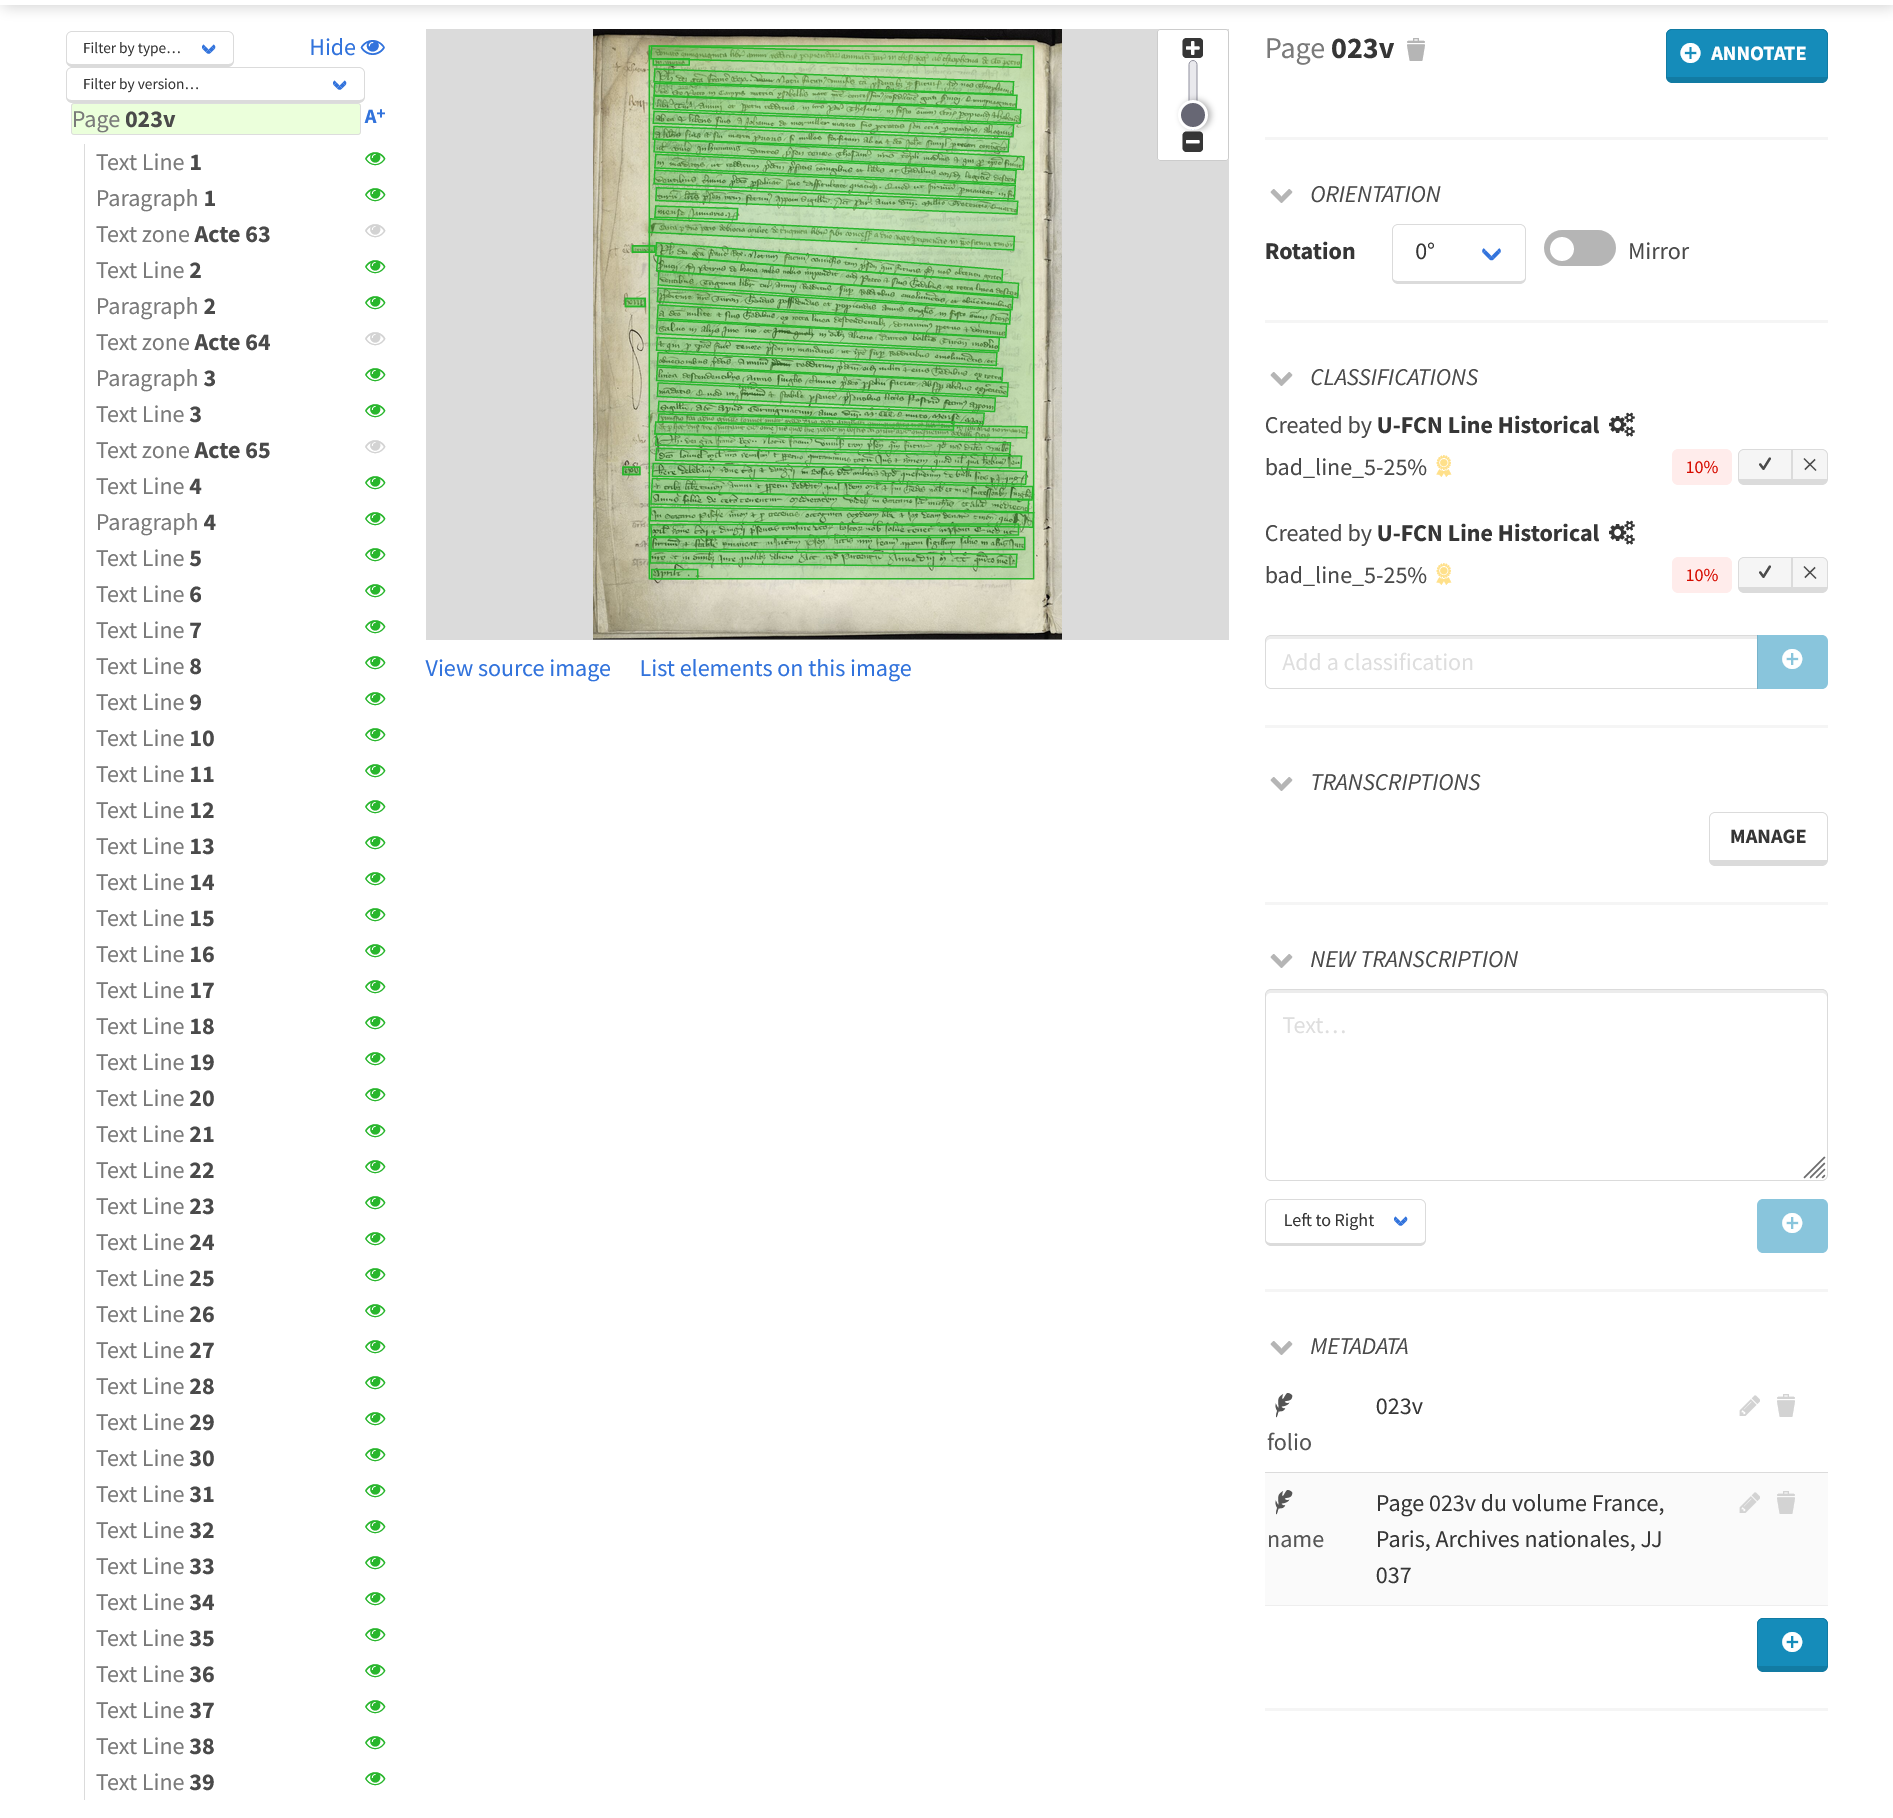
\includegraphics[width=\textwidth]{Images/Interface_Arkindex.png}
		\caption{Segmentation initiale des pages dans la plateforme Arkindex. L'élément page comprend à gauche les éléments enfants, au centre l'image de la page avec les éléments "Paragraph" et "Text Line" en surbrillance et à droite les métadonnées associées à la page.}
		\label{Page_Initiale_Arkindex}
	\end{figure}
	
	
	\subsection{Des zones de texte comme interface entre actes et pages}
	
	Le texte est ici contenu par des éléments qui découlent directement des éléments pages. Or ce n'est pas ici la manière la plus pertinente d'aborder le contenu des registres. En effet la description disponible de ces derniers concerne essentiellement les actes qu'ils contiennent et non les pages. Pour faire le lien entre chaque acte et les éléments qui le concernent contenus dans l'inventaire des registres, il faut donc transformer la segmentation des zones de texte en fonction de la séparation des actes. Cette séparation ne suit que rarement celle des pages : il est fréquent qu'une page contienne plusieurs actes ou qu'un acte soit présent dans plusieurs pages. Il arrive même que les pages portant les parties d'un même acte ne soient pas à la suite les unes des autres et que d'autres actes entrecoupent ces parties.
	
	La segmentation du contenu des registres a donc été revue pour être organisée en fonction des actes qu'ils contiennent et non en fonction des pages. Il a donc été imaginé un niveau supplémentaire de segmentation au travers des zones de textes. Celles-ci correspondent aux différents composants d'un acte au sein des pages. Ils sont donc à la fois une composante des actes et des pages et forment une interface entre le contenu physique et le contenu intellectuel des registres.
	
	\section{Des métadonnées prêtes à l’import}
	
	\subsection{Alignement des données issues d'Arkindex et des inventaires}
	
	Les inventaires des registres du Trésor des Chartes\footnote{\cite{glenisson_registres_1958}. Pour une description plus précise du contenu des instruments de recherche, \textit{cf}. Chapitre 3.} ont donc été utilisés pour extraire les différentes données permettant de décrire ces actes et les aligner avec celles issues de la plateforme Arkindex. Le tout a été organisé sous la forme d'un fichier JSON au sein duquel les actes ont été ordonnés par volume puis par son rang au sein du volume.
	
	\begin{figure}
		\centering
		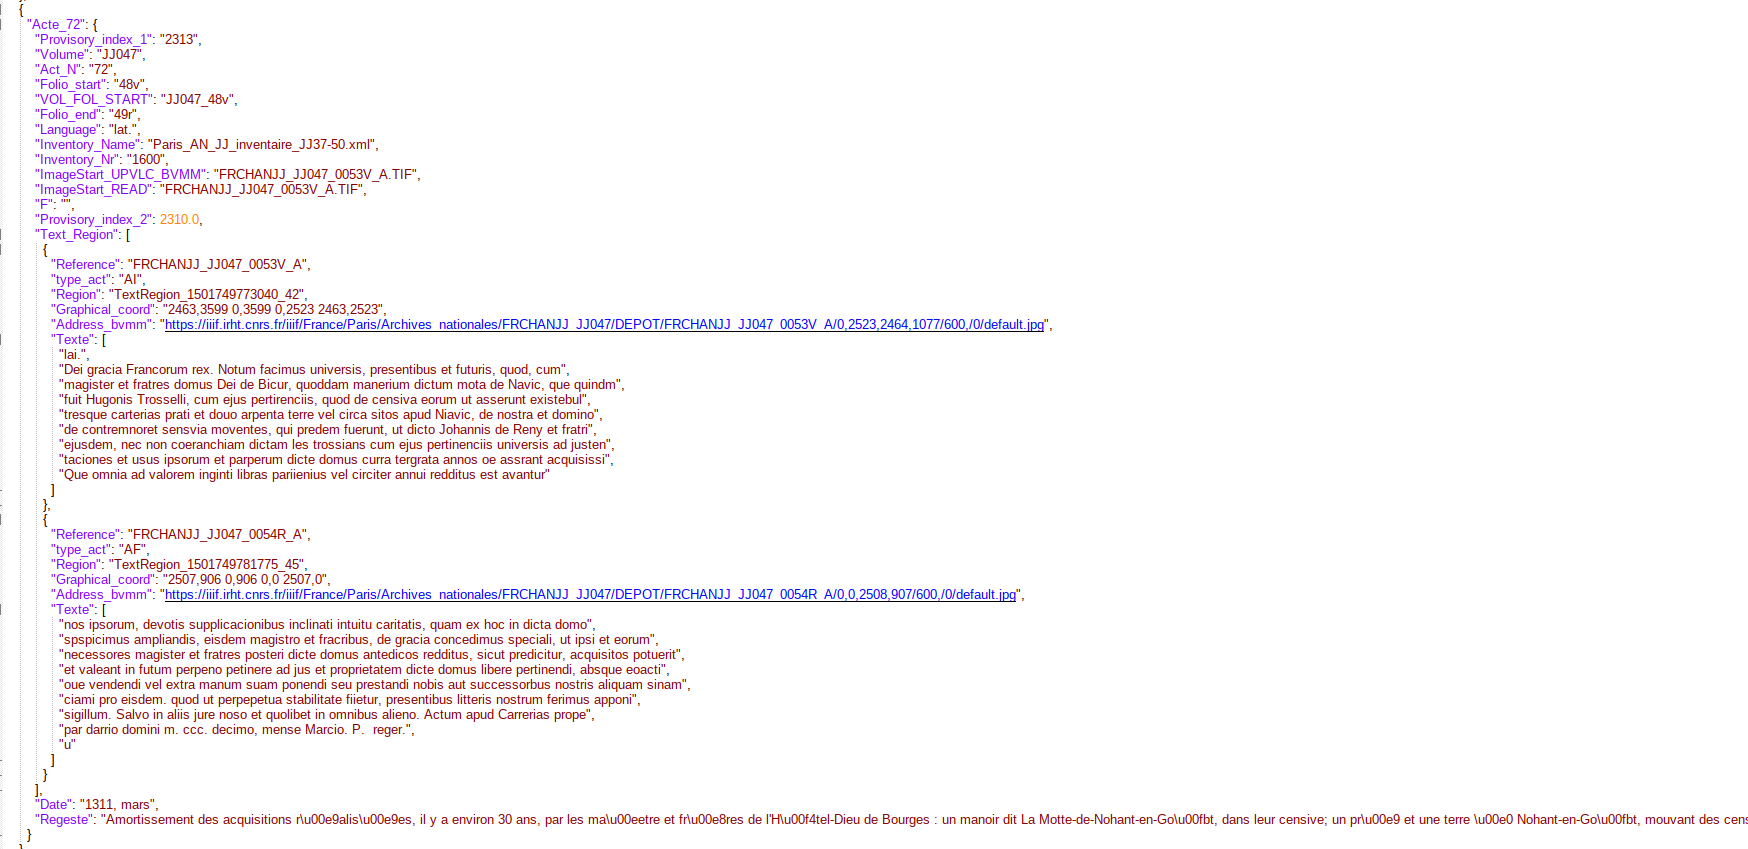
\includegraphics[width=\textwidth]{Images/json_zones_textes.png}
		\caption{Exemple d'un acte contenu par le fichier JSON sous sa forme initiale.}
		\label{json_initial}
	\end{figure}
	
	Ces actes se présentent sous la forme d'un élément dictionnaire (\textit{cf}. Figure \ref{json_initial}) dont les clefs sont le numéro du volume, le numéro de l'acte dans le volume, le folio de début de l'acte, le folio de fin de l'acte, la langue, la référence de l'inventaire, le numéro de l'acte dans cet inventaire, le nom de l'image dans la BVMM, la date, la description de l'acte par l'inventaire et plusieurs numérotations provisoires utilisées au cours de ce travail. Une dernière clef contient sous forme d'une liste de dictionnaires l'ensemble des données sur les zones de texte qui forment ces actes. Ces données sont issues de la segmentation en acte de la transcription automatique des images des manuscrits. Chaque zone de texte est composée de la transcription ligne à ligne, de la référence de l'image, des coordonnées de la zone dans l'image, de l'url correspondant à ces coordonnées et de la partie de l'acte que représente cette zone. Cette dernière métadonnée peut prendre plusieurs formes : "AC" pour les actes composés d'une seule zone de texte, "AI", "AM" ou "AF" pour les actes composés de plusieurs zones de textes successives ou "AS" pour les zones de textes qui ne sont pas à la suite des zones précédentes.
	
	\subsection{Normalisation des éléments}
	
	Afin d'envisager l'import de toutes ces données au sein d'Arkindex\footnote{Nous décrirons plus précisément ce travail au Chapitre 8}, nous avons été confrontés au problème de la normalisation des données. Par exemple, les dates peuvent se présenter sous différentes formes :
	
	\begin{quotation}
		"Date": "1317, 16 février"
	\end{quotation}
	
	\begin{quotation}
		"Date": "10 janvier 1359"
	\end{quotation}

	\begin{quotation}
		"Date": "1304-1305"
	\end{quotation}
	
	\noindent Nous avons donc écrit un script python contenant un arbre de décision pour transformer ces dates en fonction de la manière dont elles se présentent\footnote{	\url{https://github.com/virgile-reignier/Memoire-TNAH-2022-Reignier/blob/main/Scripts/Normalize_json/Normalize_date.py}.}. Une fois normalisée, la date se présente sous la forme d'une liste contenant soit un élément dictionnaire unique dans le cas d'une date précise :

	\begin{quotation}
		"Date-normalisee": [\\
		\indent\indent\{\\
		\indent\indent	"type": "when",\\
		\indent\indent	"year": 1359,\\
		\indent\indent	"month": 1,\\
		\indent\indent	"day": 10\\
		\indent\indent\}\\
		\indent ]\\
	\end{quotation}
	
	\noindent soit deux éléments dans le cas d'une intervalle :
	
	\begin{quotation}
				"Date-normalisee": [\\
				\indent\indent		\{ \\
				\indent\indent		"type": "notBefore",\\
				\indent\indent		"year": 1304,\\
				\indent\indent		"month": null,\\
				\indent\indent		"day": null\\
				\indent\indent	\},\\
				\indent\indent	\{\\
				\indent\indent		"type": "notAfter",\\
				\indent\indent		"year": 1305,\\
				\indent\indent		"month": null,\\
				\indent\indent		"day": null\\
				\indent\indent	\}\\
				\indent	]\\
	\end{quotation}
	
	\noindent Un certain nombre de formes uniques ont également été repérées au cours de cette étape puis normalisées manuellement, comme par exemple :
	
	\begin{quotation}
		"Date": "1323, 3 septembre (corriger 13 septembre ?)"
	\end{quotation}

	\noindent La normalisation des langues a suivi un processus similaire car elles se présentaient initialement sous plusieurs formes :
	
	\begin{quotation}
		"Language": "lat. et fr."
	\end{quotation}

	\begin{quotation}
		"Language": "francais"
	\end{quotation}
	
	\pagebreak
	
	\noindent Nous avons ici aussi rédigé un script python pour normaliser ces données sous une forme unique\footnote{\url{https://github.com/virgile-reignier/Memoire-TNAH-2022-Reignier/blob/main/Scripts/Normalize_json/Normalize_language.py}.}. Le résultat se présente donc sous la forme d'un élément dictionnaire contenant la norme utilisée\footnote{Pour la liste des codes décrits par la norme iso-639-3, \textit{cf}. \url{https://fr.wikipedia.org/wiki/Liste_des_codes_ISO_639-2}.} et la liste des langues reconnues encodées en fonction de cette norme :
	
	\begin{quotation}
				"normalized\_language": \{\\
			\indent\indent "norme": "iso-639-3",\\
			\indent\indent "language": [\\
			\indent\indent\indent "lat",\\
			\indent\indent\indent "frm"\\
			\indent\indent]\\
			\indent\}
	\end{quotation}
	
	\noindent La dernière étape de ce travail consistait à revoir les numérotations provisoires établies précédemment. Le contenu du fichier a en effet été modifié au cours du temps, ce qui a affecté leur forme. L'attribut "provisory\_index\_2" s'est ainsi trouvé avec une valeur vide à plusieurs reprises. Au contraire, des valeurs "bis" ont été ajoutées à l'attribut "provisory\_index\_1" qui n'est donc pas complètement linéaire :
	
	\begin{quotation}
		"Provisory\_index\_1": "8774"
	\end{quotation}
	
	\begin{quotation}
		"Provisory\_index\_1": "8774bis"
	\end{quotation}

	\begin{quotation}
		"Provisory\_index\_1": "8775"
	\end{quotation}
	
	\noindent Nous avons donc créé un nouvel attribut "Provisory\_index\_3" permettant d'associer chaque acte à un entier unique correspondant à son rang dans le fichier :
	
	\begin{quotation}
		"Provisory\_index\_3": 8774
	\end{quotation}

	\begin{quotation}
		"Provisory\_index\_3": 8775
	\end{quotation}
	
	\begin{quotation}
		"Provisory\_index\_3": 8776
	\end{quotation}

	\begin{figure}
		\centering
		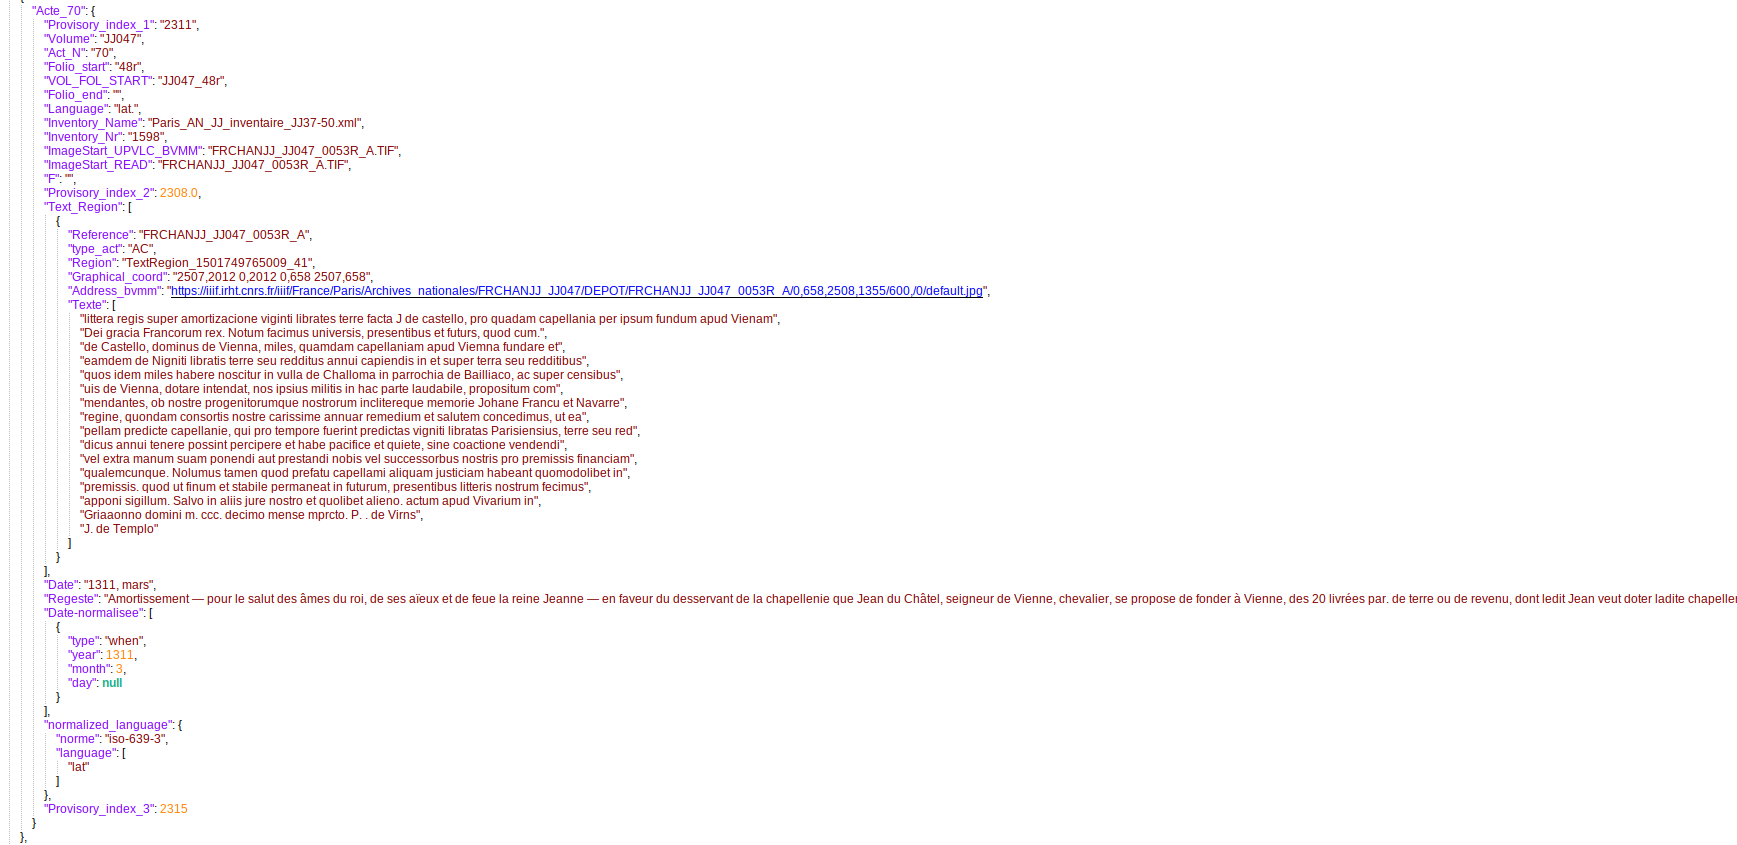
\includegraphics[width=\textwidth]{Images/json_modifie.png}
		\caption{Exemple d'un acte contenu par le fichier JSON après normalisation des éléments}
		\label{json_final}
	\end{figure}
	
	
	\section*{Conclusion}
	
	En conséquence, ce chapitre nous a permis d'aborder les différents éléments disponibles grâce aux recherches réalisées au sein du projet Himanis. Ces travaux ont aboutis au développement de modèles de REM et de REN qui ont ensuite été appliqués pour transcrire automatiquement les registres du Trésor des Chartes. La transcription obtenue a été segmentée en fonction des actes contenus dans les registres, puis alignée avec les données présentes dans les inventaires décrivant ces mêmes actes. Après quelques modifications réalisées pendant le stage, nous disposons maintenant d'un fichier complet décrivant l'ensemble du contenu des registres inventoriés de ce corpus. La Figure \ref{json_final} présente un exemple du format final des actes décris dans ce fichier.
	
	
	\chapter{\textit{Legacy Metadata} : numérisation et exploitation des instruments de recherche}
	
	Comme nous l'avons vu, le projet Himanis s'est appuyé à plusieurs reprises sur les instruments de recherche qui concernent le Trésor des Chartes, que ce soit pour la construction du modèle de REM à partir des éditions de Paul Guérin ou pour la description du contenu des registres à partir des inventaires systématiques. Ces instruments de recherche sont autant de données disponibles pour appréhender le contenu des registres. Conçus selon une structure logique facilement identifiable, ces outils de travail se prêtent à la numérisation pour être utilisés dans le cadre de traitements numériques de la donnée. Ces \textit{legacy data} fournissent ainsi toute une série de métadonnée clé-en-main pour entraîner des modèles de lecture automatique des registres.
	
	Ce chapitre sera donc consacré à l'utilisation des instruments de recherche du Trésor des Chartes dans le cadre du projet Himanis. Nous présenterons dans un premier temps les différents outils disponibles et leurs lacunes. Puis nous exposerons les transformations réalisées à partir de ces ouvrages afin de structurer leur contenu sous format numérique. Pour finir, nous décrirons le projet de structuration de l'index dans lequel notre stage s'est inséré.
	
	\section{Description du matériel disponible}
	
	\subsection{Inventaires systématiques et géographiques}
	
	Corpus incontournable pour étudier le pouvoir des rois de France à la fin du Moyen Âge, le Trésor des Chartes a été l'objet de nombreuses études qui ont permis d'en diffuser largement le contenu. Ces travaux ont été complétés par plusieurs projets archivistique de description systématique des registres pour faciliter l'accès au contenu de ce fonds\footcite{stutzmann_recherche_2017}. L'outil le plus complet et le plus précis est l'inventaire analytique des Registres du Trésor des Chartes publié par les Archives Nationales sous la direction de Robert Fawtier entre 1958 et 1999\footcite{glenisson_registres_1958}. Il propose une analyse systématique des actes contenus dans les registres JJ 37 à JJ 79B avec le rang de l'acte dans l'inventaire, les dates de temps et de lieu, un résumé de l'acte et de potentiels renvois (\textit{cf}. Figure \ref{inventaire_papier}).
	
	\begin{figure}
		\centering
		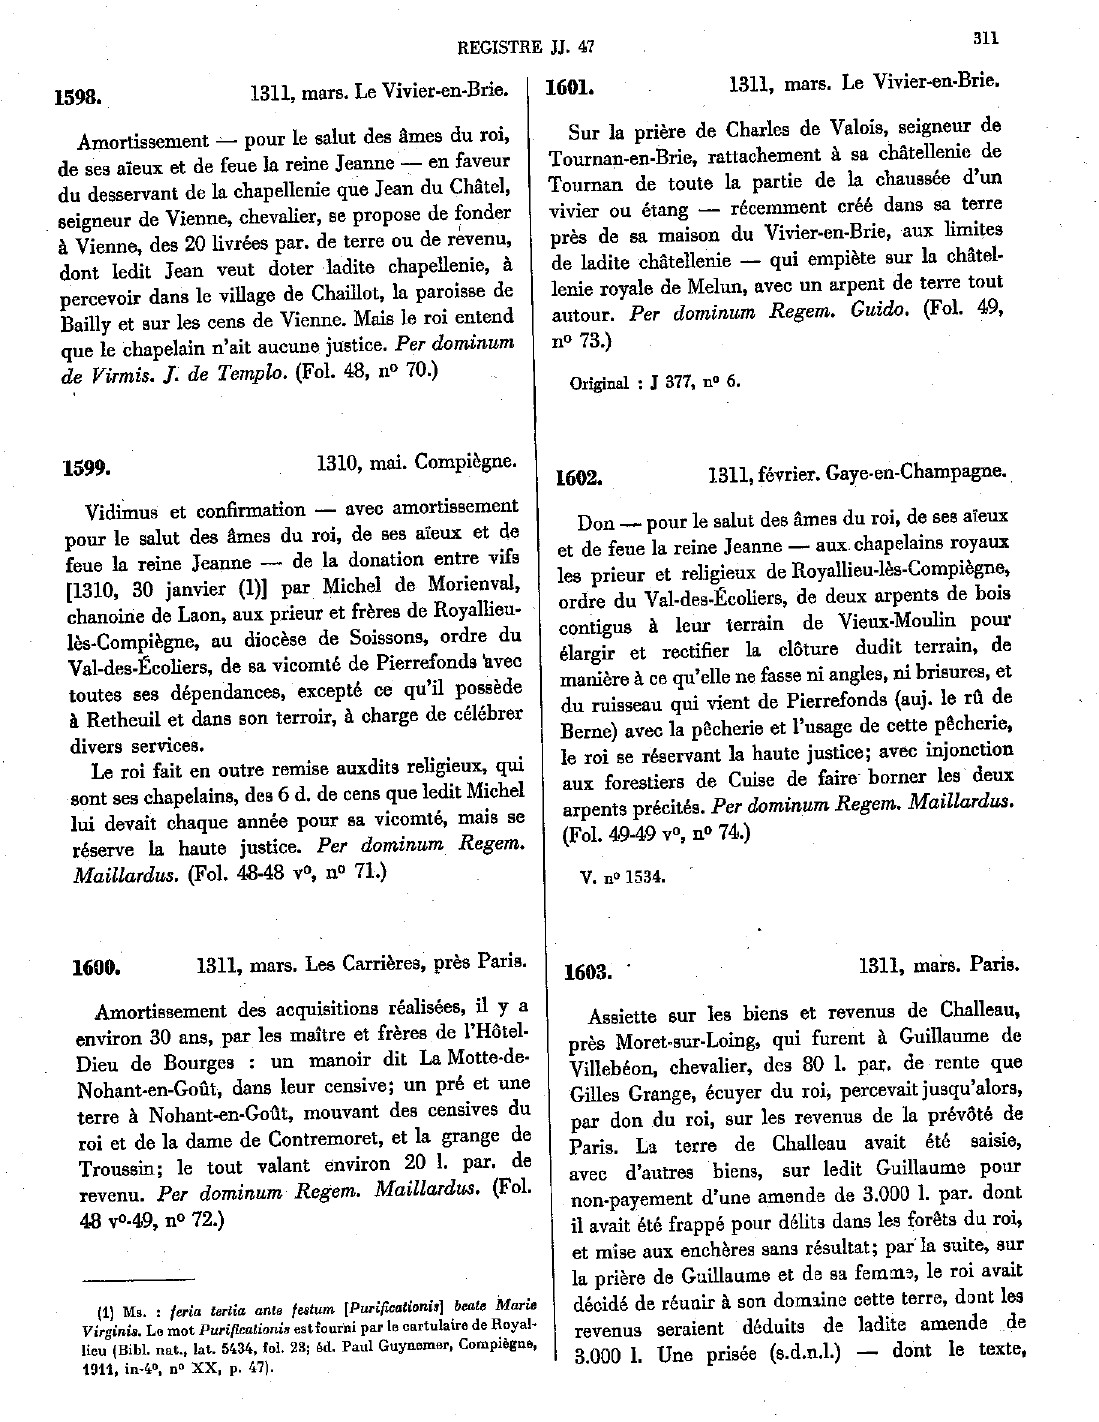
\includegraphics[width=\textwidth]{Images/Inventaire_papier.jpg}
		\caption{Exemple d'analyses contenues dans l'inventaire des registres du Trésor des Chartes publié sous la dir. de Robert Fawtier.}
		\label{inventaire_papier}
	\end{figure}
	
	Ces ouvrages disposent également d'une suite sous forme manuscrite ou dactylographiée pour les registres JJ 80 à JJ 98 réalisée par Y. Lanhers, A. Vallée, S. Clémencet et P. Luc entre 1945 et 1985\footnote{Archives Nationales, IR 49 à IR 59, IR 5127 et IR 50000.}. Le travail d'inventaire systématique ne recouvre cependant pas l'ensemble du corpus et les seuls instruments disponibles pour les registres de la fin du Moyen Âge sont les inventaires thématiques qui recensent systématiquement les actes selon un axe précis. Les plus complets sont trois inventaires géographiques rassemblant les actes qui concernent la Gascogne, le Languedoc, le Rouergue et la Loire Moyenne\footcite{samaran_gascogne_1966, dossat_languedoc_1983, chevalier_les_1993}.
	
	\subsection{Documentation complémentaire : inventaires papier, éditions et indexations}
	
	Un autre moyen de compléter ces lacunes est d'utiliser les instruments de recherche anciens dressés au XVIII\ieme\ siècle et complétés au XIX\ieme. Leur consistance est cependant assez faible puisqu'ils se contentent de compiler les tables des actes contenues dans les registres\footnote{Inv. ms. de JJ 1 à JJ 264, dressé au début du XVIIIe s., révisé et complété par A. Longnon et A. Coulon, 1880-1900, copie en quatre vol., IR421-IR424 et IR 429 ; Acta omissa. Inv. somm. ms. de la série JJ, actes non mentionnés dans	l’inv. de A. Longnon et A. Coulon, 1898-1900, IR33-IR34.}. On retrouve également des informations précieuses dans les éditions partielles des actes du Trésor des Chartes. Outre celle de Guérin que nous avons déjà citée, il en existe 4 autres consacrées à Amiens, Paris pendant le règne de Philippe VI et la Normandie et Paris pendant l'occupation anglaise au début du XV\ieme\ siècle\footcite{guerin_actes_1881, viard_documents_1899, longnon_paris_1878, le_cacheux_actes_1907, maugis_documents_1908}. Un autre moyen d'accéder au contenu des registres est d'utiliser un index des sujets, noms de personnes et noms de lieux. La plupart des ouvrages que nous venons de citer en contiennent, à l'exception notable du tome II de l'inventaire analytique des registres du Trésor des Chartes pour lequel un index des noms de lieux est en préparation. Enfin, deux instruments permettent d'aborder les actes des registres à partir des noms de lieux, personnes et sujets pour les registres de Charles VI et Henri VI\footnote{Archives Nationales, IR 1810 et Projet d'inventaire par C. Gut, 2010.}. Ils sont disponibles respectivement sous forme de fiches papiers et d'un fichier texte. 
	
	Ainsi donc, le matériel disponible pour étudier ce corpus est à la fois conséquent et très lacunaire. Alors que des pans entiers sont connus de manière précise grâce aux inventaires systématiques et géographiques, un grand nombre de registres ne disposent que d'instruments très primaires pour repérer le contenu qui intéresse le chercheur et éviter un dépouillement systématique de ces archives. L'automatisation de l'analyse archivistique est donc un enjeu essentiel pour faire progresser la recherche sur le pouvoir du roi de France en facilitant la lecture des registres et les dépouillements ponctuels et précis.

	\section{Formats de l’information}
	
	\subsection{Segmentation en XML}
	
	Un certain nombre des outils que nous avons décrits ont déjà été numérisés et convertis par les Archives Nationales sous format EAD, une norme utilisant le langage XML (\textit{Extensible Markup Language}) pour structurer des descriptions de manuscrits ou de documents d’archives. Ils présentent cependant quelques variations dans leur format, c'est pourquoi les membres du projet Himanis ont fait ici le choix de tout transformer sous un format homogène utilisant la norme TEI, un autre format basé sur le langage XML. L'objectif est de pouvoir combiner les transcriptions des textes avec les métadonnées les concernant\footcite{stutzmann_recherche_2017}.
	
	\begin{figure}
		\centering
		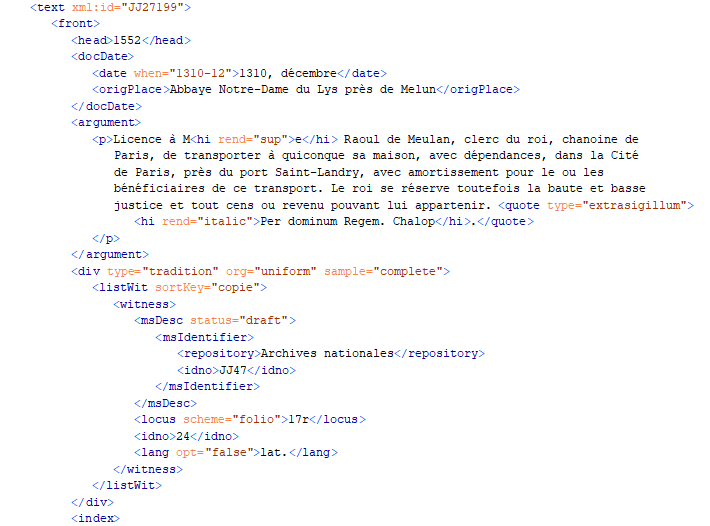
\includegraphics[width=\textwidth]{Images/Inventaire_en_TEI.png}
		\caption{Exemple d'analyse d'un acte du Trésor des Chartes encodée sous format XML-TEI.}
		\label{inventaire_TEI}
	\end{figure} 
	
	Comme présenté par la Figure \ref{inventaire_TEI}, chaque acte y est encodé au sein d'un élément <text> disposant d'un attribut @xml:id permettant de lui associer un identifiant unique. Les balises enfants contiennent ensuite le rang de l'acte dans l'inventaire, les dates de lieu et de temps, l'analyse du texte et sa manifestation physique dans les registres du Trésor des Chartes. Les fichiers ont par la suite été mis en ligne dans le répertoire Github du projet\footnote{\url{https://github.com/oriflamms/himanis/tree/master/Inventories}.} et leur contenu a servi à la constitution d'un fichier sous format JSON décrivant les actes des registres inventoriés\footnote{\textit{Cf}. Chapitre 2.}.
	
	\subsection{Numérisation de l’index}

	Ce travail de segmentation du contenu des instruments de recherche pour l'organiser sous le format XML-TEI a également été réalisé pour les différents index qui accompagnent ces ouvrages. Chaque entrée est insérée dans une balise <p> qui peut contenir une ou plusieurs balises <seg> en fonction du nombre de sous-entrées présentes. L'entité et sa description sont ensuite insérées dans une balise <term> et les renvois vers les actes décrits par l'index sont rassemblés dans une balise <num>. Chaque renvoi est ensuite inséré dans une balise <idno> (\textit{cf}. Figure \ref{index_TEI}).
	
	\begin{figure}
		\centering
		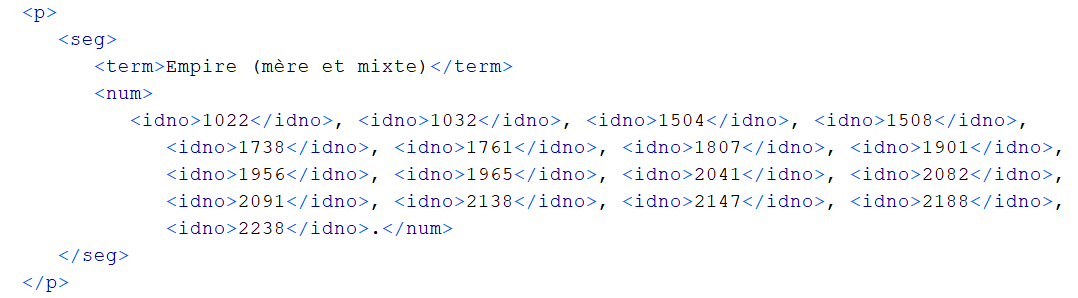
\includegraphics[width=\textwidth]{Images/index_en_TEI.png}
		\caption{Exemple d'une entrée d'index encodée sous format XML-TEI.}
		\label{index_TEI}
	\end{figure} 
	
	Une des difficultés de ce travail a été de reconstituer les sous-entrées de l'index. Le corps de certaines est en effet directement dépendant de celui de l'entrée principale, ce qui rend délicat sa manipulation comme une entité isolée. Par exemple l'entrée
	
	\begin{quotation}
		Récupérations : des arrérages de bois
	\end{quotation}

	\noindent est suivie de la sous-entrée
	
	\begin{quotation}
		des droits royaux
	\end{quotation}

	\noindent Cette dernière n'a pas de sens prise isolément, il faut donc ici reconstituer la notion dans son ensemble : "Récupérations des droits royaux". Ce travail de reconstitution a été réalisé en s'appuyant autant que possible sur la structure de l'index : les ":" servent ici de séparateur entre l'entrée principale et les sous-entrées, tandis que ces dernières sont systématiquement séparées par un "; — ". Le travail réalisé a donc consisté à éliminer le premier séparateur et à transformer le second en " , — " afin de bien marquer les entrées dont le corps dépend de celui d'une entrée générale. Pour les cas exposés, la segmentation en TEI donne le résultat suivant :
	
	\begin{quotation}
		<term>Récupérations des arrérages de bois</term>
	\end{quotation}

	\begin{quotation}
		<term>Récupérations , — des droits royaux</term>
	\end{quotation}

	\section{Les index comme compléments aux métadonnées décrivant les actes ?}

	\subsection{Le projet : mettre à plat les entrées d’index}
	
	L'objectif de ce travail était ainsi de faciliter l'association de chaque entrée d'index aux entrées d'inventaire qui lui correspondent. En effet, le but du processus était d'utiliser cet index comme vérité terrain pour développer l'apprentissage du liage d'entités. L'index a donc été mis à plat en fonction de cette logique : toutes les balises <idno> dans les entrées d'index ont été utilisées pour identifier l'entrée d'inventaire contenant la notion décrite par cette entrée. Afin que le lien soit bien manifeste, les entrées d'inventaires décrites en TEI ont été enrichies d'une balise <index> contenant l'ensemble des entrées d'index renvoyant vers l'acte en question. La Figure \ref{index_in_inventaire} donne un exemple de ces entrées d'index encapsulées dans des éléments <term> et disposant d'un attribut @type dont la valeur est "place", "person" ou "subject" en fonction du type d'entrée dont il s'agit\footnote{A propos de la typologie des entrées, \textit{cf}. Chapitre 4.}.
	
	\begin{figure}
		\centering
		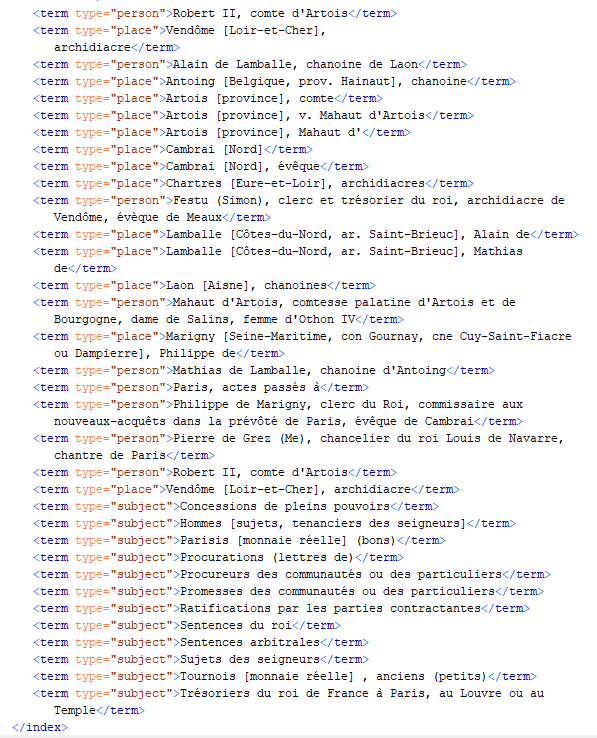
\includegraphics[width=\textwidth]{Images/Index_in_inventaire.png}
		\caption{Exemple d'une liste d'entrées d'index contenue dans une balise <index> insérée dans l'entrée d'inventaire sous format XML-TEI qui lui correspond.}
		\label{index_in_inventaire}
	\end{figure} 
	
	Le projet était d'inscrire directement les entrées d'index au sein des métadonnées de l'acte afin qu'elles puissent être comprises comme autant d'entités nommées contenues dans le texte. Cela devait faciliter l'association entre texte et entités nommées et façonner la vérité terrain permettant l'apprentissage du liage d'entités. Cette vision de l'index mis à plat comme une extension de l'inventaire jointe aux métadonnées des actes a largement guidé la segmentation des entrées car il fallait que chacune se suffise à elle-même pour qu'on puisse la comprendre comme une entité nommée à reconnaître.
	
	\subsection{Perte de qualité et de complexité dans les données}
	
	Cette vision des choses n'est cependant pas sans poser quelques problèmes dans la mise en œuvre du liage d'entités. L'index ainsi mis à plat correspond en effet moins à une base de connaissances proprement dite qu'à un ensemble d'entités nommées associées au texte. Elle ne permet pas l'apprentissage du liage puisqu'elle ne se fonde pas sur un référentiel en tant qu'entité autonome du texte. Les entités nommées sont ici simplement répétées au lieu où elles ont été reconnues et ne disposent pas de métadonnées pour les décrire (définition du concept, synonymes, coordonnées géographiques, ...). L'absence de référentiel unique et autonome ne permet donc pas le traitement a posteriori des entrées pour les segmenter en différentes parties ou les enrichir par alignement avec d'autres référentiels. C'est ainsi que l'absence d'identifiant unique pour les entrées d'index condamne le travail à rester dans l'état où il est au moment de la mise à plat alors que le liage d'entités peut aussi conduire à augmenter le nombre d'entités nommées identifiées dans les textes.
	
	De plus, l'index se caractérise par un ensemble de relations entre les entrées : associations entre entrées générales et sous-entrées, renvois contenus dans les données, ou encore entrées rejetées vers une autre entrée. Or ces relations, qui ne peuvent être reportées par la mise à plat de l'index, sont essentielles à plusieurs titres pour construire le travail de liage d'entités.  Par exemple, les entrées rejetées ne contenant pas de renvois vers l'inventaire mais uniquement un renvoi vers une autre entrée d'index sont complètement invisibilisées lors de ce travail de mise à plat alors qu'elles fournissent autant d'alias d'une même notion mobilisables au moment de la construction de la base de connaissances. De même les renvois contenus dans les entrées et les relations entre entrées générales et sous-entrées permettent d'appréhender l'association entre les entités et les possibles synonymies ou co-occurences de celles-ci, elles sont donc nécessaires à la bonne réalisation du liage. Il apparaît donc que le fait d'appréhender l'index comme un ensemble de métadonnées associées aux actes ne fournit pas un cadre optimal à la mise en œuvre du liage d'entités. La bonne compréhension du projet initial en vue duquel les données ont été manipulées est cependant essentielle pour saisir l'enjeu des étapes déjà réalisées et aborder celles que nous avons menées pour tenter d'avancer dans une direction plus propice à la constitution d'un référentiel.
	
	\section*{Conclusion}
	
	En conséquence, nous avons vu que le Trésor des Chartes dispose d'un certain nombre d'instruments de travail permettant d'appréhender les actes contenus dans les registres. Ces ouvrages sont une mine d'information pour développer la lecture automatique des textes puisqu'ils fournissent un grand nombre de métadonnées permettant de les décrire. Les membres du projet Himanis ont donc travaillé à leur numérisation et leur segmentation pour les inclure dans un modèle sous format XML-TEI. Cette transformation a placé l'acte comme élément central de description du corpus, chacun d'entre eux étant associé à l'ensemble des métadonnées disponibles pour le décrire. Ce travail a cependant trouvé sa limite au moment de la mise à plat de l'index comme devant accompagner l'ensemble de métadonnées. Les entrées d'index ne peuvent en effet pas se réduire à un ensemble d'entités nommées reconnues dans un texte et doivent constituer un référentiel propre afin de modéliser la complexité de leur définition et de leurs relations entre elles et avec les textes, puis assurer l'entraînement du liage d'entités à partir de données d'entraînement. Nous avons donc consacré un temps conséquent du stage à travailler sur ces entrées d'index pour comprendre leur complexité et la meilleure manière de la prendre en compte pour leur utilisation future.
	
	\chapter*{Conclusion partielle}
	
	Cette première partie nous a permis d'exposer dans son ensemble le contexte de travail dans lequel nous avons réalisé notre stage. Notre développement a commencé par un premier chapitre consacré à l'état de l'art sur le liage d'entités et son utilisation dans l'étude des documents patrimoniaux. Ensuite, nous avons dédié un second chapitre à la description des différentes étapes du projet Himanis et des résultats disponibles pour poursuivre le travail sur le liage d'entités. Nous avons enfin terminé cet exposé par un troisième chapitre portant sur l'utilisation des instruments de recherche disponibles comme \textit{legacy metadata} permettant de décrire le contenu des registres ainsi que les limites de cette logique.
	
	Tout cela nous a permis de voir à quel point le projet Himanis fournit un terreau favorable au développement du liage d'entités. Cette technique est en effet difficile à mettre ne œuvre pour des documents anciens car elle nécessite une base de connaissances dédiée. Or les instruments de recherches déjà numérisées par les acteurs du projet Himanis facilitent largement la constitution de cette base de connaissances. Les index disponibles se prêtent à la constitution d'un référentiel vers lequel pointer au moment de la réalisation du liage. En plus de fournir un matériel idéal pour l'entraînement d'un modèle, le Trésor des Chartes dispose également de tout un ensemble de textes non-indexés qui se prêtent à la mise en œuvre et à l'évaluation de ce modèle.
	
	\parttext{Le stage que nous avons réalisé s'est principalement concentré sur la constitution d'un référentiel pouvant servir de base de connaissances pour la mise en œuvre du liage d'entités. Nous consacrerons donc cette deuxième partie au travail de modélisation et de formalisation du référentiel à partir d'un index papier, activité qui a occupé la majeure partie de notre stage. Nous nous sommes concentrés ici sur l'index du premier volume de l'inventaire analytique des registres du Trésor des Chartes portant sur les registres JJ 37 à JJ 50 et paru en 1958. Pour rendre compte de ce travail, nous décrirons dans un premier chapitre les différentes difficultés rencontrées pour comprendre et manipuler cet instrument de recherche. Puis nous dédierons un second chapitre à l'analyse des relations entre les entités. Nous consacrerons enfin un troisième chapitre à la transformation de l'index en une base de données relationnelle.}
	
	\part{Modéliser et formaliser un référentiel à partir d’un instrument de recherche papier}
	
	
	\chapter{Appréhender les \textit{legacy data}}
	
	La mobilisation d'un instrument de travail papier pour construire un référentiel numérique implique de bien prendre le temps d'appréhender les données que l'on utilise. Leur structuration peut en effet suivre une logique complexe, passant de l'utilisation de caractères séparateurs à un grand nombre de renvois implicites. Or cette utilisation n'est pas toujours systématique et la quête de la perfection peut parfois demander un temps de relecture très conséquent pour repérer toutes les erreurs et incohérences qui peuvent se glisser dans les données de manière plus ou moins systématique. Dans le cadre de ce travail, l'index que nous avons manipulé est un ouvrage imprimé qui a été numérisé, transcrit par OCR et déjà préalablement structuré sous la forme d'un fichier au format XML-TEI. Nous avons donc consacré un temps conséquent à comprendre les différentes étapes de ce travail\footnote{\textit{Cf}. Chapitre 3.} et leur influence sur l'état des données. Ce temps est nécessaire pour faire le lien entre le fichier que nous avons manipulé et le contenu intellectuel de l'index que nous voulons reporter dans le référentiel.
	
	Ce chapitre sera donc consacré aux différentes difficultés auxquels nous avons été confrontés dans l'analyse de ces \textit{legacy data} et aux solutions mises en œuvre pour y faire face. Pour cela, nous décrirons dans un premier temps les différents type de contenus présents dans les entrées. Puis nous reporterons les différentes exceptions qu'il nous a fallu traiter tout au long de notre travail. Enfin, nous nous intéresserons aux différentes erreurs qui ont pu être mis au jour tout au long de cette chaîne de traitement.
	
	\section{Des entrées composées de différents éléments}
	
	\subsection{Reconnaître la typologie}
	
	Au début de notre stage, le fichier contient 20136 balises <term> correspondant à tous les éléments contenus dans l'index. Ces éléments se répartissent en plusieurs catégories. On retrouve tout d'abord quelques éléments titres qui sont nécessaires à l'organisation de l'index mais qui n'appartiennent pas au contenu :
	
	\begin{quotation}
		<term>INDEX DES MATIÈRES</term>
	\end{quotation}

	\begin{quotation}
		<term>A</term>
	\end{quotation}

	\noindent Nous avons ici profité de l'étape de création d'identifiants uniques pour éliminer ces éléments de la suite du processus\footnote{Nous traiterons cette étape plus précisément au Chapitre 5.}. Nous avons cependant profité auparavant de l'indication offerte par ces titres au sujet de la séparation entre les deux contenus de l'index. Celui-ci est en effet constitué d'abord d'un index des matières qui recense tous les sujets mentionnés dans les actes, puis d'un index des noms de personnes et de lieux. 
	
	Cette séparation a servi de base à l'établissement d'une typologie des entrées. Toutes les entrées présentes dans l'index des matières ont été associées au type "subject" tandis que les entrées de l'index des noms de personnes et de lieux ont dû être analysés pour discriminer celles qui relèvent du type "person" et celles qui relèvent du type "place". Cette dernière étape avait déjà été anticipée avant le début de mon stage à partir d'un principe simple : les entrées disposant de crochets ont été marquées comme des "place" et celles n'en disposant pas comme des "person". Cela donne ainsi le résultat suivant : 
	
	\begin{quotation}
		<term type="place">Montreuil [Pas-de-Calais]</term>
	\end{quotation}

	\begin{quotation}
		<term type="person">Montreuil (Pierre de)</term>
	\end{quotation}

	\noindent Si cette séparation est pertinente dans la plupart des cas, il arrive cependant que cela conduise à un certain nombre d'erreurs :
	
	\begin{quotation}
		<term type="place">Dreux (Jean) [à Orléans]</term>
	\end{quotation}
	
	\begin{quotation}
		<term type="person">Agulhou (pièce de terre dite), dans le territoire de
			Béziers</term>
	\end{quotation}
	
	\noindent Nous avons donc tenté de repérer les erreurs systématiques qui peuvent exister dans ces données. Pour cela, nous avons cherché toutes les occurrences de "terre", "bien", "bois", "près", ... pour rétablir la valeur de l'attribut @type vers "place". Un autre problème systématique concerne les personnes dont le nom renvoi vers un toponyme :
	
	\begin{quotation}
		<term type="place">Aigues-Vives [Lot-et-Garonne, con Monclar, cne Saint-Pastour?]
			(Bérenger d')</term>
	\end{quotation}

	\noindent Nous avons ici fait le choix de considérer ces noms comme relevant du type "person"\footnote{Sur les différentes formes de noms de personnes, \textit{cf}. Chapitre 5.}. Nous avons utilisé l'expression régulière "[A-Z].* de$\backslash$)" (et ses déclinaisons avec "d'", "des", ...) pour les repérer et avons procédé par une méthode semi-automatisée pour les transformer une à une tout en gardant un regard sur cette transformation afin d'éviter les effets de bords pouvant toucher les quelques exceptions de nom de lieux correspondant à ce modèle, comme par exemple :
	
	\begin{quotation}
    	<term type="place">Bannes (mas de) [Aveyron, ar. et con Villefranche-de-Rouergue,
			cne Morlhon-le-Haut]</term>
	\end{quotation}
	
	\noindent Les autres erreurs repérées ont été corrigées ponctuellement au fur et à mesure de leur identification au cours de notre travail. Il est possible qu'il en existe encore.
	
	\subsection{Segmentation des entrées}
	
	Une fois ce travail réalisé et l'index mis sous forme de tableau\footnote{Nous décrirons plus précisément les différentes étapes de traitement de l'index au Chapitre 6.}, nous avons pu repérer le contenu des entrées pour en segmenter les différentes parties en fonction du type de données. Nous avons donc rédigé un script python permettant de réaliser cette étape de manière automatisée\footnote{\url{https://github.com/virgile-reignier/Memoire-TNAH-2022-Reignier/blob/main/Scripts/Index/simplification_entrées.py}.}. Les éléments mis entre crochets ont ainsi été ajoutés dans une colonne "Détails" et ceux qui sont précédés d'une virgule dans la colonne "Supplément". Cette étape a également permis de construire une colonne "Entrée\_simplifiée" construite à partir de l'entrée originelle après extraction des éléments utilisés pour les autres colonnes. L'entrée 
	
	\begin{quotation}
		Chambre aux Deniers, Camera Denariorum [terme encore employé à cette époque pour 	désigner la Chambre des Comptes]
	\end{quotation}

	\noindent a été transformée sous la forme suivante :

	\begin{quotation}
		\begin{tabular}{|p{4cm}|p{4cm}|p{4cm}|}
			\hline
			Entrée\_simplifiée & Détails & Supplément \\ \hline
			Chambre aux Deniers & aux Deniers	terme encore employé à cette époque pour désigner la Chambre des Comptes & Camera Denariorum \\ \hline
		\end{tabular}
	\end{quotation}
	
	\noindent Cette étape a également été accompagnée d'une rationalisation des sous-entrées afin d'éviter la répétition inutile des éléments contenus dans les entrées génériques. L'entrée
	
	\begin{quotation}
		Cens cotage [acquitté pour un tènement en roture] , — morts [ne comportant pas de lods et ventes]
	\end{quotation}

	\noindent a ainsi été simplifiée afin que la colonne "Entrée\_simplifiée" devienne
	
	\begin{quotation}
		Cens cotage , — morts
	\end{quotation}

	\noindent Les données ainsi segmentées sont disponibles dans le tableau contenant les données de l'index et mis en ligne sur le Github du projet Himanis\footnote{\url{https://github.com/oriflamms/himanis/blob/master/Inventories/Systematic/Paris_AN_JJ_inventaire_JJ37-50_index.xlsx}.}.
	
	\section{Comment utiliser des \textit{semi-structured data} ?}
	
	\subsection{Des cas spécifiques tout au long de la chaîne de traitement}
	
	\subsection{Analyse fine des caractères}
	
	On a déjà parlé de structure au chapitre 3
	
	\section{Multiplication des erreurs avec l’allongement de la chaîne de traitement}
	
	\subsection{Erreurs originelle, erreurs d’OCR}
	
	\subsection{Erreurs manuelles, erreurs automatiques}
	
	
		Il y a deux articles de Caroline Parfait sur l'influence de l'OCR dans la NER
	
	Article sur l'influence de la qualité d'OCR dans l'entity linking : 
	https://hal.archives-ouvertes.fr/hal-02557116/document
	
	Thèse Yoann Dupont parle de la structure des entités nommées et de du modèle en relation des entités (intéressant par rapport à ce qu'on a fait avec Heurist)
	
	Je sais plus si j'en parle ailleurs dans mon plan, mais pour la notion de legacy data, il faut aussi voir Scheitauer (aussi pour la REN d'ailleurs)
	
	Pour la suite, sur le chapitre sur l'alignement d'entités géographiques avec Geonames et DicoTopo, ça peut être intéressant et sur le parsing des noms de lieux : https://hal.archives-ouvertes.fr/hal-02141257
	-> + ça parle aussi du lien noms personnes / lieux et des difficultés avec les lieux non-anglais et non-modernes
	
	\chapter{Analyser le lien entre les entités}
	
	Ici il faut parler de l'étape de création des identifiants qui a éliminé certaines données (cf début chapitre 4 et les entrées de noms avec un renvoi implicite.)
	
	\chapter{Transformer l’index en une base de données relationnelle}
	
	Il faut ici parler des différentes étapes et de la mise en table du modèle avant le passage par la BD relationnelle.
	
	\part{Alignement, diffusion et utilisation du référentiel}
	
	\chapter{Enrichir les données à l’aide d’un référentiel externe}
	
	On parlera ici de la segmentation des toponymes pour en extraire les différentes parties comme on a segmenté les entrées.
	
	\chapter{Mise à disposition d'un nouveau référentiel ?}
	
		Nous avons donc créé des éléments "Act" comme des enfants direct des registres et contenant tous les morceaux de textes d'un même acte. Ces éléments sont eux-mêmes composés d'éléments "Text zone" qui contiennent les morceaux de ces actes dans les pages, ils sont les enfants à la fois des éléments "Act" et des éléments "Page". Ces "Text zone" sont à l'interface entre le contenu physique et le contenu intellectuel des registres puisqu'ils représentent la manifestation des textes dans une page.
	
	\begin{figure}
		\centering
		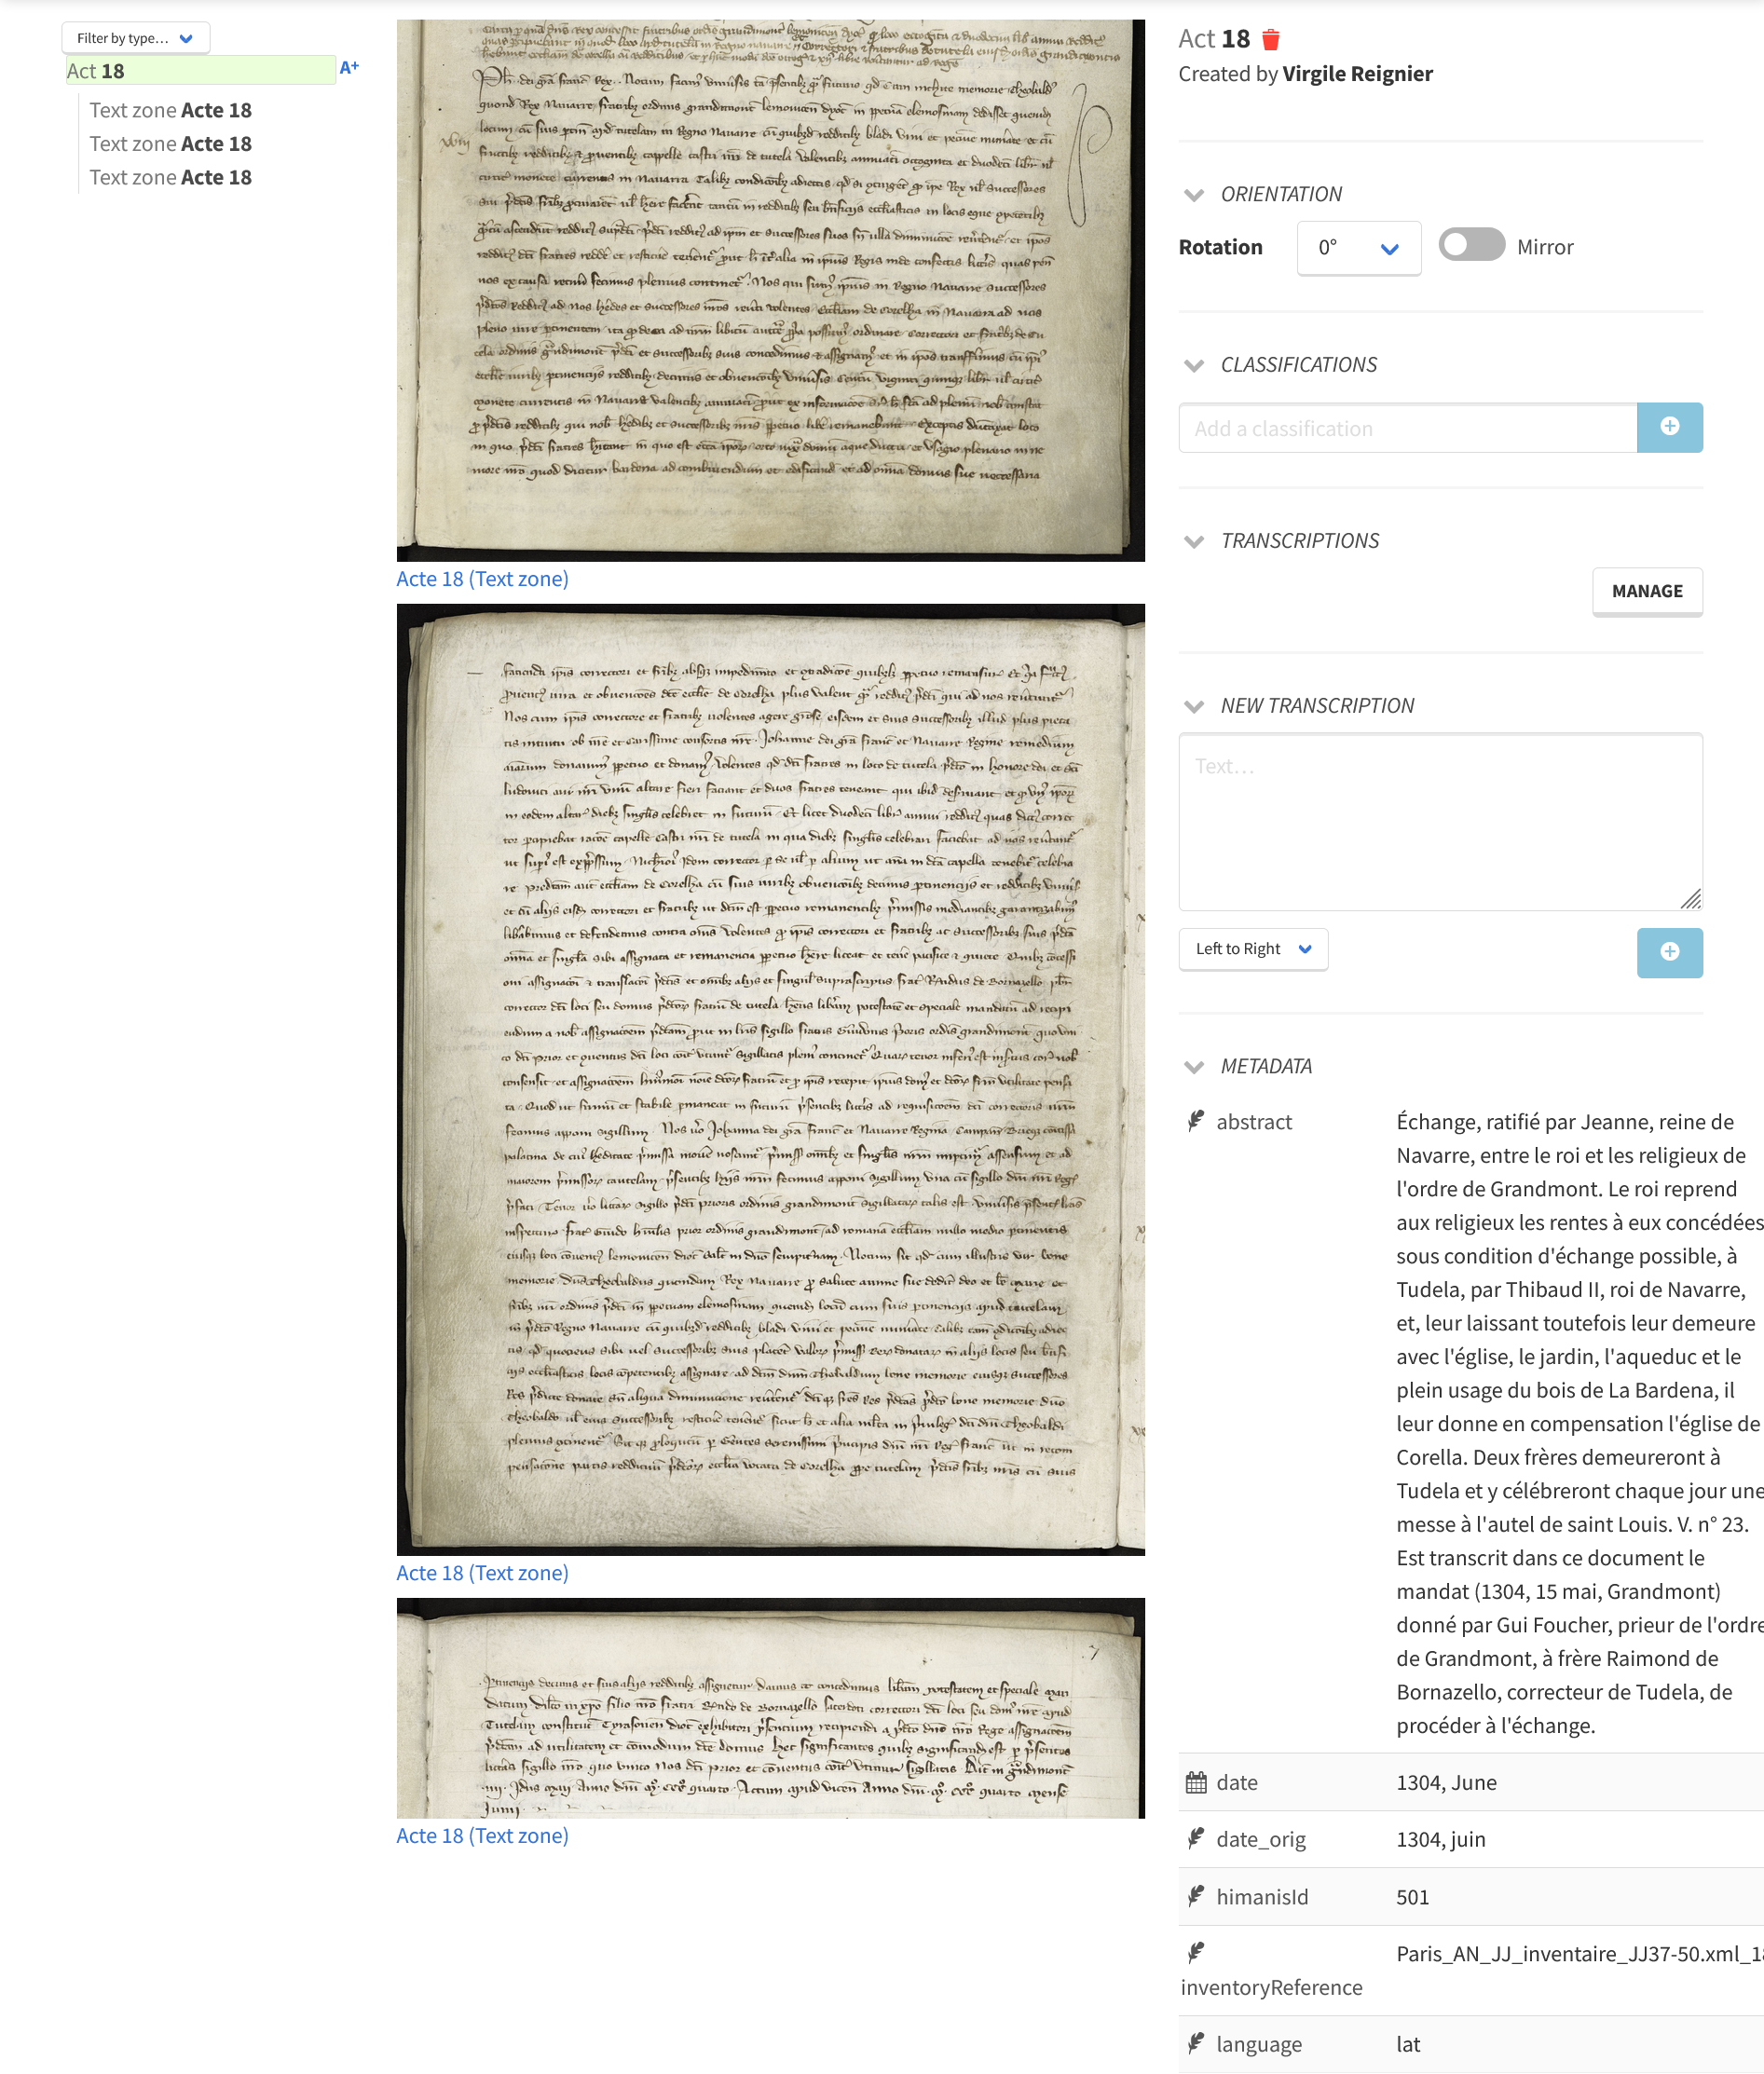
\includegraphics[width=12cm]{Images/Act_on_Arkindex.png}
		\caption{Visualisation d'un élément "Act" dans Arkindex. Cet élément est le parent de plusieurs éléments "Text zone" qui représentent chacun une portion du texte décrit par l'élément "Act".}
		\label{Act_on_Arkindex}
	\end{figure}
	
	\chapter*{Conclusion générale}
	
	Tout ce qui suit ce sont des conseils de Lucence Ing, utile à garder pour le moment mais il faudra les supprimer.
	
	\chapter{Un autre chapitre}
	
	\section{Structuration du mémoire}
	
	Le mémoire se structure en plusieurs parties :
	\begin{enumerate}
		\item tout d'abord, les pièces liminaires : page de titre, résumé, remerciements, bibliographie, introduction
		\item ensuite, le corps du texte, suivi d'une conclusion
		\item après, les annexes (documentation, extraits de code, etc.)
		\item enfin, les pièces finales : index (si besoin), glossaire (si besoin) ; tables (des figures et des tables, si nécessaire) ; table des matières
	\end{enumerate}
	
	Ce mémoire s'accompagne d'une autre partie très importante : les \textbf{données}.
	
	\section{Les données}
	
	Elles constituent une partie primordiale du travail à rendre. Ce sont :
	\begin{itemize}
		\item les données traitées (textes, images, vidéos, BDD, etc.)
		\item les scripts de traitement
		\item la documentation associée aux données et au script
		\item tout autre document qui semble nécessaire au traitement du sujet.
	\end{itemize}
	
	Ces données doivent être ordonnées et accompagnées d'un fichier \texttt{lisezMoi} (format \texttt{.txt} ou \texttt{.md}), présent à la racine du dossier contenant les données. Ce fichier doit décrire l'arborescence des fichiers et dossiers et la fonction de chacun des fichiers.
	
	Le principe important à retenir est celui de la \textbf{reproductibilité} du travail.
	
	\part{Une autre partie}
	
	
	\chapter*{Conclusion}
	\addcontentsline{toc}{chapter}{Conclusion}
	
	%les annexes
	\appendix
	\chapter{Première annexe}
	
	\backmatter
	
	\tableofcontents
	
\end{document}